\chapter{Aprendizaje automático y profundo}

	\section{Perceptrón}
	
		Ya en el año 1958, el psicólogo Frank Rosenblatt propuso un modelo llamado perceptrón el cual estaba basado en el comportamiento y funcionamiento de las neuronas de un humano, y que podía aprender ponderando cada coeficiente de entrada a la neurona \cite{historiaIA}. Hoy en día, tal y como se mostrará en esta sección, el perceptrón es la unidad fundamental de muchos modelos de \textit{machine learing} y \textit{deep learning}. \\
		
		Como se verá durante esta sección, este modelo ayuda a solucionar problemas de clasificación supervisada. Se dispone de una serie de valores de entrada $x_1, x_2, \hdots, x_n$ y se tiene una serie de valores de salida $y_1, y_2, \hdots, y_m$ que representan a qué clase pertenece la entrada ($2^m$ clases posibles). Esto se consigue mediante la ayuda de sus parámetros, que son una serie de pesos $w_1, w_2, \hdots, w_n$ y un sesgo o \textit{bias} $b$; y sus hiperparámetros, entre los que se encuentra una función $f$ de activación. \\
		
		\begin{figure}[!h]
			\centering
			\begin{tikzpicture}
				\foreach \i in {1, 2}
					\pgfmathsetmacro{\resta}{int(\i - 1)}
					\node[circle, draw, fill=gray!20] (x-\i) at (0, -1 * \resta - \resta) {$x_{\i}$};
				\node (dots) at (0, -4) {$\vdots$};
				\node[circle, draw, fill=gray!20] (x-3) at (0, -6) {$x_{n}$};
				\node[circle, draw, fill=gray!20] (n) at (5,-3) {$n_1$};
				\node[circle, draw, fill=gray!20] (a) at (7,-3) {$a_1$};
				\node[circle, draw, fill=gray!20] (b) [below = of n] {$b_1$};
				\node[circle, draw, fill=gray!20] (y) [right = of a] {$y_1$};
				
				\foreach \i in {1, 2}
					\draw[-] (x-\i) -- (n) node [midway, above, sloped] {$w_{\i}$};
				\draw[-] (x-3) -- (n) node [midway, below, sloped] {$w_n$};
				\draw[-] (n) -- (a);
				\draw[-] (a) -- (y);
				\draw[-] (b) -- (n) node [midway, right] {$1$};
			\end{tikzpicture}
			\caption{Arquitectura de un perceptrón}
			\label{fig:perceptron}
		\end{figure}
		
		En la \Cref{fig:perceptron} se muestra la arquitectura del caso más simple de un perceptrón. Se tienen $n$ entradas y una única salida. La primera parte del diagrama representa que tal y como decía Rosenblatt, cada valor de entrada debe multiplicarse por un cierto peso, de tal forma que si se representa esto en función de sus valores en un instante $k$, lo que se computa en el nodo $n_1$ es la siguiente operación. 
		
		$$
		n_1(k) = b_1(k) + \sum_{i=1}^n x_i(k)w_i(k)
		$$
		
		Una vez se ha realizado este cálculo, el valor pasa por una función de activación en el nodo $a_1$, pues esta arquitectura es común utilizarla para clasificar una entrada y es muy útil obtener una salida binaria donde se active únicamente la salida que represente la clase a la que pertenece la entrada dada. Aunque existen diferentes funciones de activación para las neuronas, al trabajar con un perceptrón, la función de activación por excelencia es la función escalón de Heaviside, donde $\mathcal{U}: \mathbb{R} \longrightarrow \{0, 1\}$ y su expresión analítica es
		
		$$
		\mathcal{U}(x) = \left\{\begin{array}{ccc}
			0 & \text{si} & x < 0\\
			1 & \text{si} & x \geq 0
		\end{array}
		\right..
		$$
		
		Combinando ambas expresiones, se puede resumir en que la salida del perceptrón es equivalente a la siguiente ecuación: 
		
		$$
		y_1(k) = \left\{\begin{array}{ccc}
			0 & \text{si} & b_1(k) + \displaystyle\sum_{i=1}^n x_i(k)w_i(k) < 0\\
			1 & \text{si} & b_1(k) + \displaystyle\sum_{i=1}^n x_i(k)w_i(k) \geq 0
		\end{array}
		\right.
		$$
		
		Para dar un ejemplo claro de cómo funciona el perceptrón, se pueden tomar una serie de observaciones que tengan dos valores de entrada y uno de salida. Además, se supondrá que existen dos clases. Esto a fin de cuentas es asignar un valor de 0 o 1 a cada punto de $\mathbb{R}^2$ tal y como se describe en la \Cref{fig:labeled_data}. \\
		
		\begin{figure}[!h]
			\centering
			\begin{tikzpicture}
				\begin{axis}[ymin = -2.5, ymax = 2.5, xmax = 2.5, xmin = -2.5, xticklabel = \empty, yticklabel = \empty, minor tick num = 1, axis lines = middle, xlabel = $x$, ylabel = $y$]
					\addplot[only marks, mark = *] coordinates {(1, 2)};
					\addplot[only marks, mark = triangle*] coordinates {(-1, 2) (0, -1)};
				\end{axis}
			\end{tikzpicture}
			\caption{Puntos etiquetados en $\mathbb{R}^2$}
			\label{fig:labeled_data}
		\end{figure}
		
		Una solución rápida sería trazar una recta $r: ax + by + c = 0$ que separe $\mathbb{R}^2$ en dos regiones, de forma que todo punto que pertenezca a una región pertenece entonces a una misma clase, tal y como se observa en la \Cref{fig:separated_label_data}. Esta recta suele llamarse \textit{decision boundary} o frontera de decisión. El problema entonces es hallar la recta $r$, pero se cumple que para este ejemplo es de la forma $w_1 x + w_2 y + b = 0$, siendo el problema encontrar los parámetros adecuados del modelo. La idea puede extrapolarse a diferente tamaño de entrada tomando un hiperplano de la forma $\textbf{w}^T \textbf{x} + b = 0$. \\
		
		Las preguntas a resolver ahora son, ¿existen siempre dichos parámetros? ¿Cómo pueden hallarse? El propio Minsky se hizo estas preguntas en \cite{perceptrons} y se dio cuenta de que dichos parámetros sí pueden hallarse en un número finito de pasos, siempre y cuando los puntos sean linealmente separables. Un ejemplo que no es linealmente separable es el de la función \gls{xor} tal y como se muestra en la \Cref{table:xor,fig:xor}, pues no existe una recta $r$ que separe $\mathbb{R}^2$ en dos regiones de tal forma que cada región contenga puntos de una única clase, sería necesaria una frontera de decisión no lineal. \\
		
		\begin{figure}
			\centering
			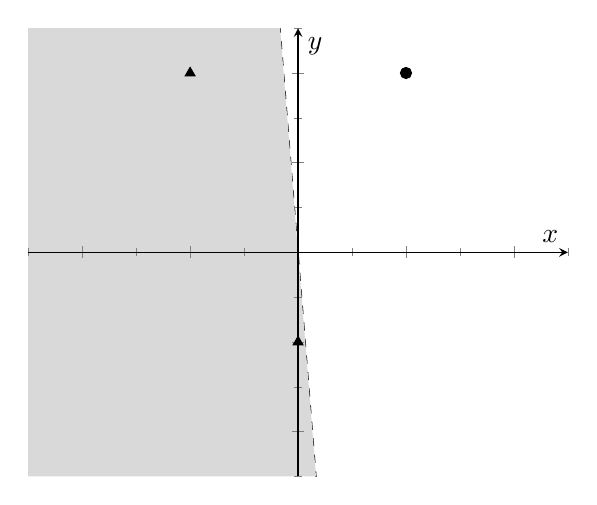
\begin{tikzpicture}
				\begin{axis}[ymin = -2.5, ymax = 2.5, xmax = 2.5, xmin = -2.5, xticklabel = \empty, yticklabel = \empty, minor tick num = 1, axis lines = middle, xlabel = $x$, ylabel = $y$, axis on top]
					\addplot[only marks, mark = *] coordinates {(1, 2)};
					\addplot[only marks, mark = triangle*] coordinates {(-1, 2) (0, -1)};
					\addplot[domain = -3:3, samples = 2, dashed] {-15*x};
					\draw[fill = gray!30, draw = none] (axis cs:-2.5, -2.5) -- (axis cs:-2.5, 2.5) -- (axis cs: -1/6, 2.5) -- (axis cs:1/6, -2.5);
				\end{axis}
			\end{tikzpicture}
			\caption{Puntos separados en $\mathbb{R}^2$}
			\label{fig:separated_label_data}
		\end{figure}
		
		\begin{table}[H]
			\centering
			\begin{tabular}{|c|c|c|}\hline
				$x$ & $y$ & $x \oplus y$\\\hline
				0 & 0 & 0\\\hline
				0 & 1 & 1\\\hline
				1 & 0 & 1\\\hline
				1 & 1 & 0\\\hline
			\end{tabular}
			\caption{Función \gls{xor}}
			\label{table:xor}
		\end{table}
		
		\begin{figure}
			\centering
			\begin{tikzpicture}
				\begin{axis}[ymin = -.5, ymax = 2.5, xmax = 2.5, xmin = -.5, xticklabel = \empty, yticklabel = \empty, minor tick num = 1, axis lines = middle, xlabel = $x$, ylabel = $y$]
					\addplot[only marks, mark = *] coordinates {(0, 0) (1, 1)};
					\addplot[only marks, mark = triangle*] coordinates {(0, 1) (1, 0)};
				\end{axis}
			\end{tikzpicture}
			\caption{Valores de $x \oplus y$ en  $\mathbb{R}^2$}
			\label{fig:xor}
		\end{figure}
		
		En cuanto a la pregunta de cómo hallar los parámetros, se consideran las siguientes ecuaciones \cite{nndesign}, donde $\textbf{w}$ es el vector de pesos, $t$ el valor esperado, y $a$ la salida del perceptrón y se aplica el \Cref{algo:perceptron} para obtener los parámetros óptimos. En dicho algoritmo se supondrá que existe una matriz $X$ de $n$ filas que contiene los diferentes $\textbf{x}$. 
		
		\begin{equation}
			\label{eq:perceptron}
			\begin{gathered}
				\textbf{w}(k+1) = \textbf{w}(k) + e(k)\textbf{x}(k)\\
				b(k+1) = b(k) + e(k)\\
				e(k) = t(k) - a(k)\\
				a(k) = \mathcal{U}(\textbf{w}^T(k)\textbf{x}(k))
			\end{gathered}
		\end{equation}
		
		
		\begin{algorithm}[!h]
			\SetProgSty{texttt}\DontPrintSemicolon
			
			\caption{Regla de aprendizaje del perceptrón}
			\label{algo:perceptron}
			
			\Datos{$X, \textbf{t}$}
			\Resultado{$\textbf{w}, b$}
			$b \gets 0$\\
			$\textbf{w} \gets$ \texttt{random}\\
			$k \gets 0$\\
			\Repetir{$\lnot$\texttt{acabar}}{
				\texttt{acabar} $\gets$ \texttt{true}\\
				\Para{$i \gets k$ \KwTo $k + n - 1$}{
					$e(i) \gets t(i) - a(i)$\\
					$\textbf{w}(i+1) \gets \textbf{w}(i) + e(i)\textbf{x}(i \pmod n)$\\
					$b(i+1) \gets b(i) + e(i)$\\
					\texttt{acabar} $\gets$ \texttt{acabar} $\land \, e(i) == 0$ 
				}
				$k \gets k + n - 1$
			}
		\end{algorithm}
		
		A cada una de las iteraciones que realiza el bucle exterior se les denomina épocas o \textit{epoch}, que consiste en realizar el proceso de entrenamiento sobre todo el conjunto de datos. En este caso se está suponiendo que no va a recibir casos que no sean linealmente separables, pero de lo contrario se puede añadir un contador \texttt{max\_epochs} y fijar un número máximo para no caer en un bucle infinito. No sería tarea fácil determinar dicho valor, pues aunque el algoritmo converge en los casos previamente explicados, no en todos lo hace de manera rápida. \\
		
		La ejecución del \Cref{algo:perceptron} para el caso de la \Cref{fig:labeled_data} finaliza tras dos épocas, donde en la primera de ellas va ajustando los pesos y el sesgo de manera adecuada, y en la segunda verifica que todas las observaciones han sido clasificadas de manera correcta. La frontera de decisión obtenida es la recta $r: 2x - 2 = 0$, que es una recta vertical. Una observación a realizar es que $\textbf{x}(1) \in r$, por tanto ¿a qué clase pertenece? Esto depende de la función de activación empleada, al utilizar $\mathcal{U}$ la clasificación es correcta, pero al cambiarla por otra, podría no serlo y necesitaría de más épocas para realizar correctamente la clasificación. \\
		
		La última cuestión que queda por tratar respecto al perceptrón es el porqué se verifica que en el caso de que los puntos dados sean linealmente separables, en un número finito de pasos, el \Cref{algo:perceptron} terminará su ejecución y con el $\textbf{w}$ óptimo, tal y como se enunciaba en el Teorema de Convergencia del Perceptrón. A continuación se presenta su demostración basándose en la que se encuentra en \cite{nndesign}, de forma más clara y simple. Para comenzar con la demostración será necesario definir una serie de elementos, comenzando por $\Omega(k)$ y $\textbf{z}(k)$.  
		
		$$
		\Omega(k) = \left(\begin{array}{c}
			\textbf{w}(k)\\\hline
			b(k)
		\end{array}\right) \,\,\, \textbf{z}(k) = \left(\begin{array}{c}
		\textbf{x}(k)\\\hline
		1
		\end{array}\right)
		 \,\,\, \Omega(0) = \begin{pmatrix}
			0\\0\\\vdots\\0
		\end{pmatrix}
		$$
		
		Con estos elementos y el cálculo de $a(k)$ en la \Cref{eq:perceptron} es fácil ver que $n(k) = \Omega^T(k)\textbf{z}(k)$. Recordando los posibles valores de $t(k)$, se deseaba que si dicho valor era 1, entonces $n(k) \geq 0$; y en caso de que valiese 0 entonces se deseaba tener $n(k) < 0$, en resumen, que $t(k) - a(k) = 0$. Otra forma de ver esto es afirmar que en el caso en que $t(k) \neq a(k)$, entonces $\Omega(k)$ debe actualizarse de acuerdo a la \Cref{eq:perceptron}. De esta forma $\Omega(k + 1) = \Omega(k) + e(k)\textbf{z}(k)$. Ahora se considerará un vector $\Omega^*$ de forma que 
		$$
		\forall k \exists \Omega^* \,\, \mathcal{U}\left(\Omega^{*^T}\textbf{z}(k)\right) = t(k),
		$$
		es decir, $\Omega^*$ es el vector de pesos óptimo. Además, por comodidad se normalizarán todas las distancias del problema, de manera que $\|\Omega^{*}\| = 1$ y $\|\textbf{z}(k)\| \leq 1$. El último elemento a considerar será $\delta$, que será definido como
		$$
		\delta = \min\left\lbrace\Omega^{*^T}\textbf{z}(i)\right\rbrace, 
		$$
		tomando además que $\delta > 0$ pues otra manera de definirlo es la distancia al punto más cercano a la frontera de decisión óptima. Con estos elementos se puede comenzar la demostración. Como la regla de actualización es $\Omega(k + 1) = \Omega(k) + e(k)\textbf{z}(k)$, al vector de pesos en un determinado instante (clasificación fallida) se le suma o resta $\textbf{z}(k)$ y a priori no se sabe cuántas veces se va a repetir esto, por lo que la idea de la demostración será ver si la norma del vector de pesos tiene una cota superior e inferior, es decir, se para de sumar o restar otros vectores $\textbf{z}(i)$, de manera que el algoritmo terminaría. Para obtener esto basta con comparar el comportamiento de $\Omega^T(k) \Omega^*$ frente a $\Omega^T(k)\Omega(k)$ (es decir, $\|\Omega\|^2$). \\
		
		Con el primero de los términos, al tratar de corregir un error se verifica que
		$$
		\Omega^T(k+1)\Omega^* = (\Omega(k) + e(k)\textbf{z}(k))^T \Omega^* = \Omega^T(k)\Omega^* + e(k)\Omega^{*^T}\textbf{z}(k). 
		$$
		Además, por la manera en la que se ha definido $\delta$, el segundo sumando pertenece al intervalo $(-\infty, -\delta] \cup [\delta, \infty)$, pudiendo deducir la siguiente desigualdad, por lo que en una actualización el término sólo varía por lo menos en $\delta$ unidades.  
		
		\begin{equation}
			\label{eq:inf_delta}
			\Omega^T(k+1)\Omega^* \geq \Omega^T(k)\Omega^* + \delta
		\end{equation}
		
		De la misma manera que se ha analizado el comportamiento de $\Omega^T(k) \Omega^*$ se procede con la actualización de $\Omega^T(k)\Omega(k)$. 
		
		\begin{align*}
			\Omega^T(k+1)\Omega(k+1) &= (\Omega(k) + e(k)\textbf{z}(k))^T(\Omega(k) + e(k)\textbf{z}(k))\\
			&= \Omega^2(k) + (e(k)\textbf{z}(k))^2 + 2e(k)\Omega^T(k)\textbf{z}(k)\\
			&= \Omega^T(k)\Omega(k) + e^2(k)\textbf{z}^T(k)\textbf{z}(k) + 2e(k)\Omega^T(k)\textbf{z}(k)\\
			&= \Omega^T(k)\Omega(k) + e^2(k)\textbf{z}^T(k)\textbf{z}(k) + 2e(k)n(k)
		\end{align*}
		
		En el segundo sumando se tiene que siempre será menor o igual que 1, pues por definición $0 \leq \textbf{z}^T(k)\textbf{z}(k) = \|\textbf{z}(k)\|^2 \leq 1$. Además, el tercer sumando siempre será cero o negativo, pues en todos los casos posibles en los que $e(k) \neq 0$ se cumple que $e(k)n(k) < 0$: 
		
		\begin{itemize}
			\item Si $t(k) = 1 \land n(k) < 0$, entonces $a(k) = 0 \land e(k) > 0$
			\item Si $t(k) = 0 \land n(k) \geq 0$, entonces $a(k) = 1 \land e(k) < 0$
		\end{itemize}
		
		De esta situación se puede deducir la siguiente desigualdad, por lo que en una actualización el término sólo varía en como máximo una unidad.   
		
		\begin{equation}
			\label{eq:sup_delta}
			\Omega^T(k+1)\Omega(k+1) \leq \Omega^T(k)\Omega(k) + 1
		\end{equation}
		
		Una vez se ha observado cómo varían estos términos al actualizarlos, se puede observar qué pasaría con ellos al hacer $m$ actualizaciones. Con el resultado obtenido en las \Cref{eq:inf_delta,eq:sup_delta} se pueden deducir las desigualdades $\delta m \leq \Omega^T(m)\Omega^*$ y $\Omega^T(m)\Omega(m) \leq m$. \\
		
		Ahora al aplicar la desigualdad de Cauchy--Schwarz\footnote{Esta desigualdad afirma que $\|\textbf{u}\textbf{v}\| \leq \|\textbf{u}\|\|\textbf{v}\|$. }, el valor de $\|\Omega^*\|$, y la propiedad transitiva, se obtiene una cota superior y otra inferior (ambas recuadradas) para $\|\Omega^T(m)\|$, lo que demuestra que el número de actualizaciones es finito y que por tanto el algoritmo converge. 
		
		\begin{align*}
			\boxed{\delta m} &\leq \Omega^T(m)\Omega^* = \|\Omega^T(m)\Omega^*\|\\
			&\leq \|\Omega^T(m)\| \|\Omega^*\| = \|\Omega^T(m)\| = \sqrt{\Omega^T(m)\Omega(m)}\\
			& \leq \boxed{\sqrt{m}} 
		\end{align*}
		
		$$
		\pushQED{\qed} 
		\delta m \leq \|\Omega(m)\| \leq \sqrt{m} \,\,\, \Longrightarrow \,\,\, m \leq \frac{1}{\delta^2}\qedhere
		\popQED
		$$ 
		
		Esta última desigualdad muestra cómo existe una relación entre el número de iteraciones del algoritmo y la distancia de los datos de entrenamiento a la frontera de decisión óptima (depende únicamente de esto). Cuanto más cerca estén, mayor será el número de iteraciones necesarias. 
		
	\section{Redes neuronales artificiales}
	
		El descubrimiento del perceptrón junto con el teorema que garantizaba que cualquier conjunto de puntos linealmente separable podría ser aprendido mediante este, supuso un gran avance en la \gls{ia} al igual que una gran desilusión por parte de muchos al no poder aprender una función tan simple como la \gls{xor}. Esto causó el llamado el primer invierno de la \gls{ia}, que finalizó con la llegada de las redes neuronales multicapa y el algoritmo de la retroprogragación. \\
		
		En 1989, George Cybenko enunció y consiguió demostrar el Teorema de Aproximación Universal \cite{teoremaAproximacion}. Este afirma que dada una red neuronal con una capa de entrada, una capa oculta con suficientes neuronas, y una capa de salida; es un aproximador universal de funciones. Es decir, si existe una relación entre dos variables $\textbf{x}$ e $\textbf{y}$, entonces una red neuronal con la arquitectura mencionada y el entrenamiento adecuado, encontrará dicha relación y podrá comportarse como una función $f$ tal que $\textbf{y} = f(\textbf{x})$. Este se considera un gran resultado, pues consigue acabar con las limitaciones del perceptrón que habían generado un decaimiento por el interés en la \gls{ia}. \\
		
		\begin{figure}[!h]
			\centering
			\begin{tikzpicture}
				\node[circle, draw, fill=gray!20] (x-1) {$x_{1}$};
				\foreach \i in {2,3}{
					\pgfmathtruncatemacro{\resta}{\i - 1}
					\node[circle, draw, fill=gray!20, below = of x-\resta] (x-\i) {$x_{\i}$};
				}
				\node (dots) [below = of x-3] {$\vdots$};
				\foreach \i in {1,2,3}{
					\node[circle, draw, fill=gray!20, right = 2cm of x-\i] (a-\i) {$a^{(1)}_{\i}$};
				}
				\node (dots2) [below = of a-3] {$\vdots$};
				\node (a-4) [circle, draw, fill=gray!20, below = of dots2] {$a^{(1)}_i$};
				\foreach \i in {1,2,3}{
					\node[circle, draw, fill=gray!20, right = 2cm of a-\i] (A-\i) {$a^{(M)}_{\i}$};
				}
				\node (dots3) [below = of A-3] {$\vdots$};
				\node (x-4) [circle, draw, fill=gray!20, left = 2cm of a-4] {$x_n$};
				\node (A-4) [circle, draw, fill=gray!20, below = of dots3] {$a^{(M)}_j$};
				\foreach \i in {1,2,3,4}{
					\node [left = .6cm of A-\i] {$\cdots$};
					\foreach \j in {1,2,3,4}{
						\draw[-] (x-\i) -- (a-\j);
					}
				}
				\foreach \i in {1,2,3}{
					\node (y-\i) [circle, draw, fill=gray!20, right =  of A-\i] {$y_{\i}$};
					\draw[-] (A-\i) -- (y-\i);
				}
				\node (y-4) [circle, draw, fill=gray!20, right =  of A-4] {$y_{j}$};
				\draw[-] (A-4) -- (y-4);
				\node (dots4) [right = 1.6cm of dots3] {$\vdots$};
			\end{tikzpicture}
			\caption{Arquitectura de una red neuronal multicapa}
			\label{fig:rna}
		\end{figure}
		
		En la \Cref{fig:rna} se muestra un diagrama que resume la arquitectura de una red neuronal multicapa. Todas las salidas de una capa están conectadas con todas las entradas de la siguiente con un peso y un \textit{bias}. En el diagrama de la \Cref{fig:rna_completa} se puede observar esto en mayor detalle. Estas pueden ser utilizadas en problemas de clasificación o regresión supervisada, pero en una primera aproximación se supondrá que se está resolviendo un problema de regresión. \\
		
		\begin{figure}
			\centering
			\resizebox{\textwidth}{!}{
				\begin{tikzpicture}
					\node[circle, draw, fill=gray!20] at (4, 0) (n-1) {$n^{(1)}_{1}$};
					\node[circle, draw, fill=gray!20, below= .5cm of n-1] (b-1) {$b^{(1)}_{1}$};
					\foreach \i in {2,3}{
						\pgfmathtruncatemacro{\resta}{\i - 1}
						\node[circle, draw, fill=gray!20, below= 2 cm of b-\resta] (n-\i) {$n^{(1)}_{\i}$};
						\node[circle, draw, fill=gray!20, below= .5cm of n-\i] (b-\i) {$b^{(1)}_{\i}$};
					}
					\node[circle, draw, fill=gray!20, below left = 2 cm and 7 cm of n-1] (x-1) {$x_{1}$};
					\foreach \i in {2,3}{
						\pgfmathtruncatemacro{\resta}{\i - 1}
						\node[circle, draw, fill=gray!20, below= 2cm of x-\resta] (x-\i) {$x_{\i}$};
					}
					\node (dots) [below = .5cm of x-3] {$\vdots$};
					\node[circle, draw, fill=gray!20, below = .5cm of dots] (x-n) {$x_{n}$};
					\node (dots2) [below = .5cm of b-3] {$\vdots$};
					\node[circle, draw, fill=gray!20, below= .5cm of dots2] (n-n) {$n^{(1)}_{i}$};
					\node[circle, draw, fill=gray!20, below= .5cm of n-n] (b-n) {$b^{(1)}_{i}$};
					\foreach \i in {1,2,3}{
						\draw[-] (n-\i) -- (b-\i) node [midway, right] {$1$};
					}
					\draw[-] (b-n) -- (n-n) node [midway, right] {$1$};
					\foreach \i in {1,2,3}{
						\foreach \j in {1,2,3}{
							\pgfmathtruncatemacro{\condicion}{ifthenelse(Mod(\i, 2)==0,1,0)}
							\ifnum\condicion=1
							\draw[-] (x-\i) -- (n-\j) node [near start, above, sloped] {$w^{(1)}_{\j\i}$};
							\else
							\draw[-] (x-\i) -- (n-\j) node [near end, above, sloped] {$w^{(1)}_{\j\i}$};
							\fi
						}
					}
					\foreach \i in {1,2,3}{
						\draw[-] (x-n) -- (n-\i) node [near start, above, sloped] {$w^{(1)}_{\i n}$};
						\draw[-] (x-\i) -- (n-n) node [near end, below, sloped] {$w^{(1)}_{i\i}$};
					}
					\draw[-] (x-n) -- (n-n) node [midway, below, sloped] {$w^{(1)}_{in}$};
					\foreach \i in {1,2,3}{
						\node[circle, draw, fill=gray!20, right = 1cm of n-\i] (a-\i) {$a^{(1)}_{\i}$};
					}
					\node[circle, draw, fill=gray!20, right = 1cm of n-n] (a-n) {$a^{(1)}_{i}$};
					\foreach \i in {1,2,3}{
						\draw[-] (n-\i) -- (a-\i);
					}
					\draw[-] (n-n) -- (a-n);
					\foreach \i in {1,2,3}{
						\node [right = .7cm of a-\i] {$\cdots$};
						\node[circle, draw, fill=gray!20, right = 2cm of a-\i] (N-\i) {$n^{(M)}_{\i}$};
					}
					\node[circle, draw, fill=gray!20, right = 2cm of a-n] (N-4) {$n^{(M)}_{j}$};
					\node [right = .7cm of a-n] {$\cdots$};
					\foreach \i in {1,2,3}{
						\node[circle, draw, fill=gray!20, right = 1cm of N-\i] (A-\i) {$a^{(M)}_{\i}$};
					}
					\node[circle, draw, fill=gray!20, right = 1cm of N-4] (A-4) {$a^{(M)}_{j}$};
					\foreach \i in {1,2,3,4}{
						\draw[-] (N-\i) -- (A-\i);
					}
					\foreach \i in {1,2,3}{
						\node[circle, draw, fill=gray!20, below= .5cm of N-\i] (B-\i) {$b^{(M)}_{\i}$};
						\draw[-] (N-\i) -- (B-\i) node [midway, right] {$1$};
					}
					\node [below = .5cm of B-3] {$\vdots$};
					\node[circle, draw, fill=gray!20, below= .5cm of N-4] (B-4) {$b^{(M)}_{j}$};
					\draw[-] (N-4) -- (B-4) node [midway, right] {$1$};
					\foreach \i in {1,2,3}{
						\node[circle, draw, fill=gray!20, right = 22 cm of x-\i] (y-\i) {$y_{\i}$};
					}
					\node[circle, draw, fill=gray!20, right = 22 cm of x-n] (y-4) {$y_{j}$};
					\foreach \i in {1,2,3,4}{
						\draw[-] (A-\i) -- (y-\i);
					}
				\end{tikzpicture}
			}
			\caption{Red neuronal multicapa}
			\label{fig:rna_completa}
		\end{figure}
		
		Al igual que un perceptrón quedaba representado mediante un vector $\textbf{w}$ de pesos y un valor de sesgo $b$, para representar una red neuronal multicapa se hace mediante las matrices $W^{(m)}$ y los vectores $\textbf{b}^{(m)}$ y $\textbf{f}^{(m)}$, que contienen los pesos, los sesgos, y las funciones de activación. La notación para los sesgos es $b_i^{(m)}$, que representa el sesgo de la entrada $i-$ésima de la capa $m$. De igual manera $f_i^{(m)}$ representa la función de activación la neuona $i-$ésima de la capa $m$. Para los pesos, $w_{ij}^{(m)}$ denota el peso que une la salida $j$ con la entrada $i$ de la capa $m$. Para las capas, $1 \leq m < M$. En ningún momento un exponente entre paréntesis representa una potencia, en dicho caso aparecerá sin paréntesis para distinguirlo. Siguiendo los mismos pasos que con el perceptrón, la primera pregunta será cómo calcular la salida de una red neuronal. La salida de una capa se calcula con la \Cref{eq:prop}, teniendo en cuenta que $\textbf{x}^{(m)} = \textbf{y}^{(m-1)}$, por lo que para calcular la salida de la red no hay más que aplicar dicha ecuación hasta llegar a la última capa. 
		
		\begin{equation}
			\label{eq:prop}
			\begin{gathered}
				\textbf{a}^{(m)}(k) = \textbf{f}^{(m)}\left(W^{(m)}(k)\textbf{x}^{(m)}(k) + \textbf{b}^{(m)}(k)\right)\\
				\begin{pmatrix}
					a_1^{(m)}(k)\\a_2^{(m)}(k)\\\vdots\\a_j^{(m)}(k)
				\end{pmatrix} = \textbf{f}^{(m)}\left(
				\begin{pmatrix}
					w_{11}^{(m)}(k) & w_{12}^{(m)}(k) & \cdots & w_{1i}^{(m)}(k)\\
					w_{21}^{(m)}(k) & w_{22}^{(m)}(k) & \cdots & w_{2i}^{(m)}(k)\\
					\vdots & \vdots & \ddots & \vdots\\
					w_{j1}^{(m)}(k) & w_{j2}^{(m)}(k) & \cdots & w_{ji}^{(m)}(k)\\
				\end{pmatrix}
				\begin{pmatrix}
					x_1^{(m)}(k)\\x_2^{(m)}(k)\\\vdots\\x_i^{(m)}(k)
				\end{pmatrix} + 
				\begin{pmatrix}
					b_1^{(m)}(k)\\b_2^{(m)}(k)\\\vdots\\b_j^{(m)}(k)
				\end{pmatrix}\right)
			\end{gathered}
		\end{equation}
		
		A continuación, se puede plantear cuál es la ecuación del error para una red neuronal. Esta es simplemente cuestión de elección al igual que las funciones de activación. Al trabajar con redes neuronales para problemas de regresión, la función de error por excelencia es el error cuadrático, definido como
		$$
		L(k) = \sum(\textbf{t}(k) - \textbf{a}^{(M)}(k))^2, 
		$$
		aunque existen otras muchas, cada una adecuada a cada tipo de problema y modelo, como por ejemplo el error cuadrático medio, error absoluto, error absoluto medio, error logarítmico, error exponencial, entropía cruzada, etc \cite{funcionesError}.\\
		
		La pregunta ahora sería que, al igual que existía una ecuación para actualizar los parámetros del perceptrón ¿existe para una red neuronal? Para deducirla fácilmente, basta en pensar que $L$ es una función que depende de los parámetros de la red y que se quiere que su valor sea lo más pequeño posible para diferentes vectores de entrada, es decir, encontrar los valores de los parámetros que minimizan $L$. Esto es un problema clásico de cálculo que en el caso de una variable se resuelve igualando a cero la derivada de la función, y en el caso de varias, mediante la matriz Hessiana. Sin embargo, dichos métodos para una función de tantas variables y con expresiones complejas, no son muy eficientes. \\
		
		Esto se soluciona con ayuda de un algoritmo conocido como descenso por gradiente \cite{descenso}. Este algoritmo calcula de manera iterativa una aproximación de los mínimos de una función con ayuda del vector gradiente de una función. El vector gradiente de una función $f$ se define como 
		$$
		\nabla f(x_1, x_2, \hdots, x_n) = \left(\frac{\partial f}{\partial x_1}, \frac{\partial f}{\partial x_2}, \hdots, \frac{\partial f}{\partial x_n}\right), 
		$$
		e indica la dirección en la que la función crece más rápido, siendo la idea principal del algoritmo ir moviéndose en dirección contraria a este. 
		
		\begin{algorithm}
			\SetProgSty{texttt}\DontPrintSemicolon
			
			\caption{Descenso por gradiente}
			\label{algo:descenso}
			
			\Datos{$f, \alpha, k$}
			\Resultado{$\textbf{x}(k)$}
			$\textbf{x}(0) \gets$\texttt{ random}\\
			\Para{$i \gets 1$ \KwTo $k$}{
				$\textbf{x}(i + 1) = \textbf{x}(i) - \alpha\nabla f(\textbf{x}(i))$
			}
		\end{algorithm}
		
		Como se observa en el \Cref{algo:descenso}, se comienza en un punto aleatorio, lo que puede variar la calidad de la solución dependiendo de la ejecución, y además se introduce un término $\alpha$ llamado tasa de aprendizaje. Pueden existir casos en los que la magnitud del gradiente sea muy grande, lo que resulta en desplazamientos bruscos y una convergencia más lenta, tal y como se refleja en la \Cref{fig:descenso}. Si se hubiese fijado un valor máximo de $k = 25$, en los casos de las \Cref{fig:descenso_grande,fig:descenso_peq}, no se hubiese llegado a una buena aproximación del mínimo por haber elegido un $\alpha$ inadecuado. 
		
		\begin{figure}[H]
			\centering
			\begin{subfigure}{.3\textwidth}
				\centering
				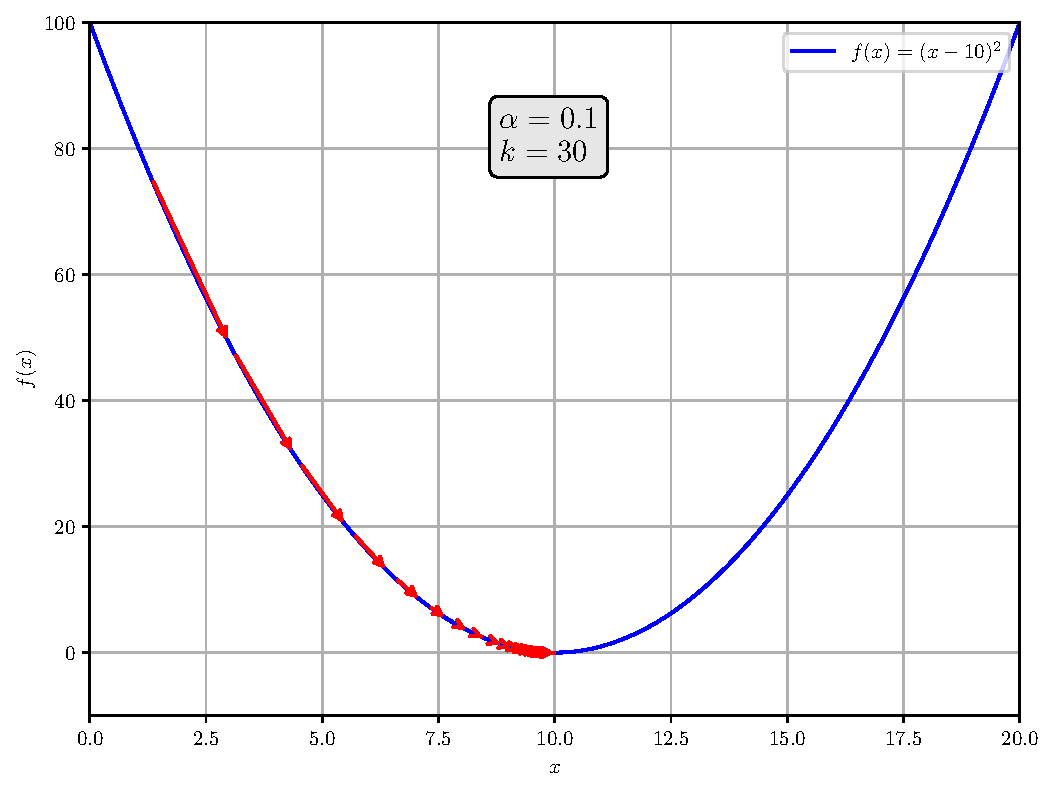
\includegraphics[width = \linewidth]{descenso}
				\caption{$\alpha$ adecuada}
			\end{subfigure}
			\begin{subfigure}{.3\textwidth}
				\centering
				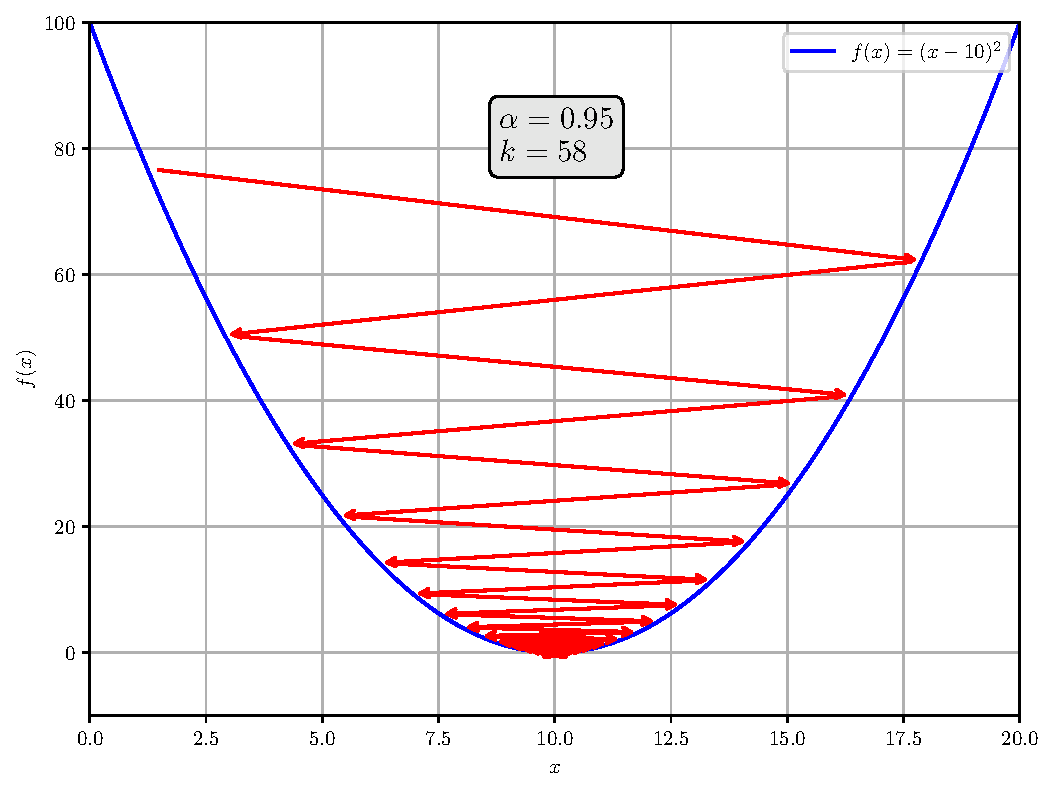
\includegraphics[width = \linewidth]{descenso2}
				\caption{$\alpha$ demasiado grande}
				\label{fig:descenso_grande}
			\end{subfigure}
			\begin{subfigure}{.3\textwidth}
				\centering
				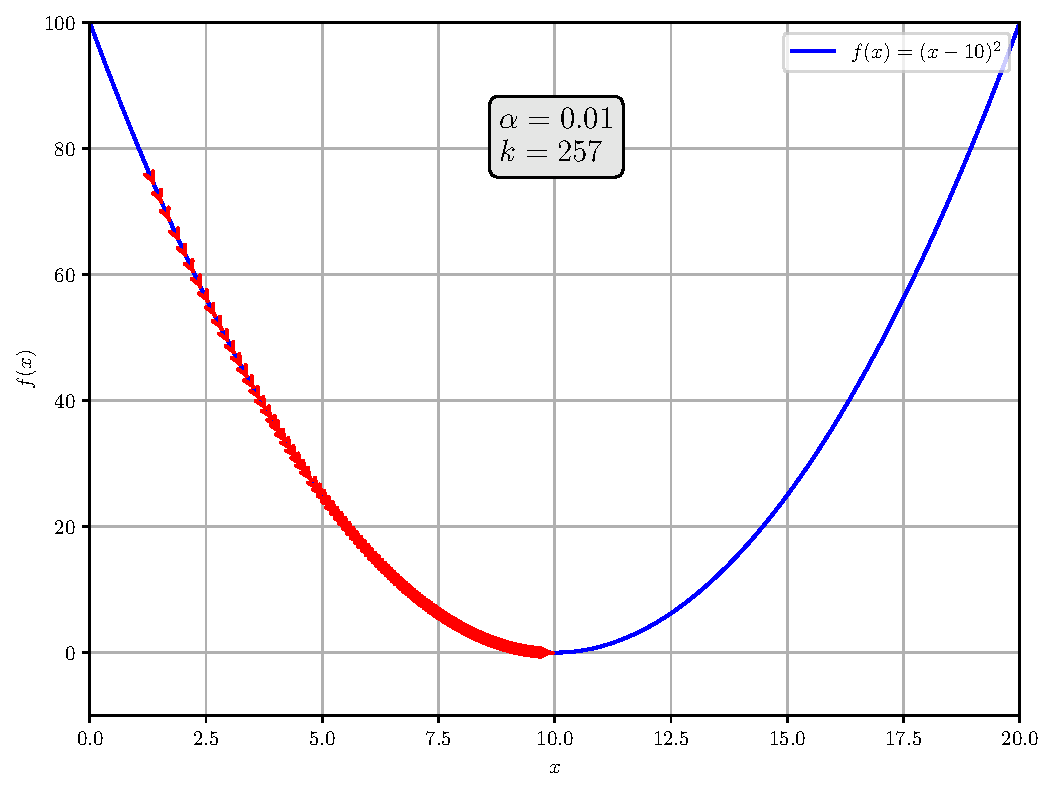
\includegraphics[width = \linewidth]{descenso3}
				\caption{$\alpha$ demasiado pequeña}
				\label{fig:descenso_peq}
			\end{subfigure}
			\caption{Descenso por gradiente}
			\label{fig:descenso}
		\end{figure}
		
		Con esta idea de la función de error y el descenso por gradiente, aparece el famoso algoritmo de la retropropagación o \textit{backpropagation}. Es muy similar al algoritmo de aprendizaje del perceptrón pero adaptado a la estructura de una red neuronal. El primer paso consiste en dada una entrada, calcular la salida de la red con ayuda de la \Cref{eq:prop}. El segundo paso es calcular el error $L(k)$. Esta función depende de todos los pesos y sesgos de la red, por lo que el tercer paso será modificar estos de acuerdo a $\nabla L$ y repetir el procedimiento para el resto de observaciones. Se realizan tantas épocas como sean necesarias. \\
		
		El problema que queda por resolver es cómo calcular todos los elementos de $\nabla L$, pues por ejemplo es fácil calcular $\frac{\partial L}{\partial a_i^{(M)}}$, pero no parece tan obvio calcular $\frac{\partial L}{\partial w_{ij}^{(m)}}$, pues hay que retroceder $M-m$ capas, y habrá muchos valores que dependan de ese peso. La solución a esto es la regla de la cadena. 
		
		$$
		\frac{\partial f}{\partial x} = \sum_{i=1}^n \frac{\partial f}{\partial u_{i1}}\frac{\partial u_{im}}{\partial x}\prod_{j=1}^{m-1}\frac{\partial u_{ij}}{\partial u_{ij+1}}
		$$
		
		Con ayuda de esta regla se pueden calcular fácilmente los términos no triviales del gradiente, propagando el error hacia atrás por la red hasta llegar al parámetro deseado mediante las sensibilidades $\left(\delta_i^{(s)}\right)$ \cite{nndesign}. De aquí se intuye el porqué del nombre del algoritmo. De manera informal, lo que hace el algoritmo es castigar a cada neurona de manera proporcional a su participación en el error final. 
		
		$$
		\begin{gathered}
			\frac{\partial L}{\partial b_{i}^{(s)}} = \frac{\partial L}{\partial a_{i}^{(s)}} \frac{\partial a_{i}^{(s)}}{\partial n_{i}^{(s)}} \frac{\partial n_{i}^{(s)}}{\partial b_{i}^{(s)}} = \delta_i^{(s)}\\
			\frac{\partial L}{\partial w_{ij}^{(s)}} = \frac{\partial L}{\partial a_{i}^{(s)}} \frac{\partial a_{i}^{(s)}}{\partial n_{i}^{(s)}} \frac{\partial n_{i}^{(s)}}{\partial w_{ij}^{(s)}} = \delta_i^{(s)} \frac{\partial n_{i}^{(s)}}{\partial w_{ij}^{(s)}} = \delta_i^{(s)} a_j^{(s-1)}\\
			\delta_i^{(M)} = \frac{\partial L}{\partial a_{i}^{(M)}} \frac{\partial a_{i}^{(M)}}{\partial n_{i}^{(M)}} = -2a_{i}^{(M)} \frac{\partial a_{i}^{(M)}}{\partial n_{i}^{(M)}} = -2a_{i}^{(M)} \frac{\partial f_{i}^{(M)}}{\partial n_{i}^{(M)}}\\
			\delta_i^{(m)} = \frac{\partial L}{\partial n_i^{(m)}} = \sum_{l=1}^p\frac{\partial L}{\partial n_l^{(m+1)}}\frac{\partial n_l^{(m+1)}}{\partial n_i^{(m)}} = \sum_{l=1}^p \delta_l^{(m+1)} \frac{\partial n_l^{(m+1)}}{\partial n_i^{(m)}} = \sum_{l=1}^p \delta_l^{(m+1)} w_{li}^{(m+1)} \frac{\partial f_i^{(m)}}{\partial n_i^{(m)}}\\
			\text{con } 0 < m < M \text{ y } 0 < s \leq M
		\end{gathered}
		$$
		
		Estas ecuaciones pueden reescribirse de manera matricial para aligerar la notación, que combinándolas con las ideas explicadas referentes al \Cref{algo:descenso}, da lugar al \Cref{algo:backprop}, bastante similar al \Cref{algo:perceptron} pero adaptado a una red neuronal. \\
		
		\begin{algorithm}
			\SetProgSty{text}\DontPrintSemicolon
			
			\caption{Retropropagación (\textit{backpropagation})}
			\label{algo:backprop}
			
			\Datos{$\textbf{f}^{(s)}, \textbf{x}^{(1)}(k), \textbf{t}(k), \varepsilon$}
			\Resultado{$W^{(s)}, \textbf{b}^{(s)}$}
			
			\Para{$i \gets 1$ \KwTo $\varepsilon$}{
				\ParaCada{$\textbf{x}^{(1)}$}{
					\texttt{calcular} $\textbf{a}^{(M)}(k)$\\
					\texttt{calcular} $L(k)$ y $\nabla L(k)$\\
					$
					\begin{gathered}
						\delta^{(M)}(k) \gets -2 \frac{\partial \textbf{f}^{(M)}}{\partial \textbf{n}^{(M)}}(\textbf{t}(k) - \textbf{a}^{(M)}(k))\\
						\delta^{(m)}(k) \gets \frac{\partial \textbf{f}^{(M)}}{\partial \textbf{n}^{(M)}} W^{(m+1)^T}(k)\delta^{(m+1)}(k)
					\end{gathered}
					$\\
					$W^{(m)}(k+1) \gets W^{(m)}(k) - \alpha \delta^{(m)}(k)(\textbf{a}^{(m-1)}(k))^T$\\
					$\textbf{b}^{(m)}(k+1) \gets \textbf{b}^{(m)}(k) - \alpha \delta^{(m)}(k)$
				}
			}
		\end{algorithm}
		
		En esta variante del algoritmo denominada \gls{sgd} se actualizan los parámetros por cada observación del \textit{dataset} y se ha decidido elegir como criterio de parada alcanzar un número de épocas, aunque también se suelen tomar otros criterios, como la magnitud del error. Además, esta variante es computacionalmente costosa, pues para cada observación se calcula el gradiente. Otra variante del algoritmo es el batch. Esta no actualiza por cada observación como \gls{sgd}, halla el gradiente del error promedio de todas las observaciones del \textit{dataset}. No es recomendable, pues es muy costosa y si el \textit{dataset} ocupa mucho, puede no caber en memoria. Ambas aproximaciones se pueden combinar para dar lugar a una variante más eficiente que estas dos, denominada mini-batch, que realiza lo mismo que \textit{batch} pero dividiendo el \textit{dataset} en \textit{minibatches} y realizando una actualización de los parámetros por cada uno de ellos. De esta manera no se necesita tener todo el \textit{dataset} en memoria \cite{descenso}. 
		
		\subsection{Funciones de activación}
		
			Durante el estudio del perceptrón, se muestra cómo se emplea la función de Heaviside como función de activación en la neurona. Esto se debe a que se busca una función que independientemente de los valores de entrada que reciba, produzca una salida binaria. En ciertos casos, no se deseará una salida binaria pues el problema no tendría porqué ser de clasificación, como se ha visto con las redes neuronales. Además, como se ha visto en el \Cref{algo:backprop}, será imprescindible poder calcular la derivada de estas funciones. Por estos motivos, se presentan las funciones de activación más conocidas e importantes \cite{funcionesActivacion,softmax}. 
			
			\begin{itemize}
				\item \textbf{Función lineal}
				
				\begin{figure}[!h]
					\centering
					\begin{tikzpicture}
						\draw[->] (-2,0) -- (2,0) node[right] {$x$};
						\draw[->] (0,-2) -- (0,2) node[above] {$f(x)$};
						
						\draw[domain = -2:2, smooth, variable = \x] plot ({\x},{\x});
						\node[right] at (1.5,2.5) {$f(x) = x$};
					\end{tikzpicture}
					\caption{Función lineal}
					\label{fig:funcion_lineal}
				\end{figure}
				
				Con motivo de emplear una función que no produzca valores binarios, se pueden tomar funciones lineales $f: \mathbb{R} \longrightarrow \mathbb{R}$ de la forma $f(x) = ax$. No es muy útil al trabajar con tareas complejas, solo es capaz de cumplir con su tarea en problemas sencillos, y esto en parte se debe a la expresión de su derivada. Al ser un polinomio, es continua y derivable en todo $\mathbb{R}$, teniendo que
				$$
				\frac{df}{dx} = a. 
				$$
				
				\item \textbf{Función logística}
				
				\begin{figure}[!h]
					\centering
					\begin{tikzpicture}
						\begin{axis}[
							xlabel = $x$,
							ylabel = {$f(x)$},
							xmin = -10, xmax = 10,
							ymin = 0, ymax = 1,
							width = 0.8\textwidth,
							height = 0.35\textwidth,
							xticklabel = \empty,
							yticklabel = \empty,
							axis lines = middle,
							domain = -10:10,
							samples = 100,
							]
							\addplot[black] {1/(1 + exp(-x))};
							\node at (axis cs: 5,0.8) {$f(x) = \frac{1}{1 + e^{-x}}$};
						\end{axis}
					\end{tikzpicture}
					\caption{Función logística}
					\label{fig:funcion_sigmoide}
				\end{figure}
				
				Esta también es una función que no devuelve valores binarios, es conocida como función sigmoide por la forma de S que tiene, y es una función $f: \mathbb{R} \longrightarrow (0, 1)$. Una propiedad que es muy útil es que es solución de la ecuación diferencial
				$$
				\frac{df}{dx} = f(x)(1 - f(x)). 
				$$
				
				Es un intento de mejora de la función de activación empleada en el perceptrón, pues una ligera variación en la entrada puede crear un gran cambio en la salida. Esta función evita que eso suceda, pues una pequeña variación en la entrada produce una variación pequeña en la salida. 
				
				\item \textbf{Tangente hiperbólica}
				\begin{figure}[!h]
					\centering
					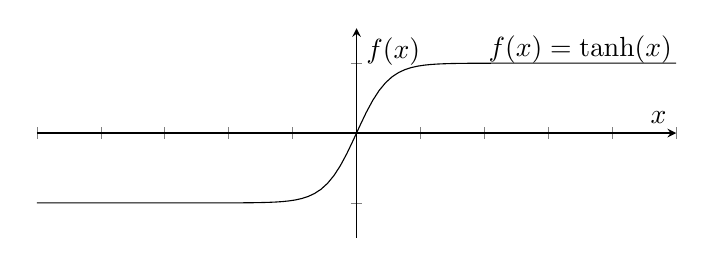
\begin{tikzpicture}
						\begin{axis}[
							xlabel = $x$,
							ylabel = {$f(x)$},
							xmin = -10, xmax = 10,
							ymin = -1.5, ymax = 1.5,
							width = 0.8\textwidth,
							height = 0.35\textwidth,
							xticklabel = \empty,
							yticklabel = \empty,
							axis lines = middle,
							domain = -10:10,
							samples = 100,
							]
							\addplot[black] {tanh(x)};
							\node at (axis cs: 7, 1.2) {$f(x) = \tanh(x)$};
						\end{axis}
					\end{tikzpicture}
					\caption{Tangente hiperbólica}
					\label{fig:funcion_tanh}
				\end{figure}
				
				De nuevo, esta función no devuelve valores binarios, y que guarda cierta relación con la logística, pues esta tiene también forma de sigmoide, pero a diferencia que la logística, esta verifica que $f(-x) = -f(x)$ por lo que es preferible sobre esta, y también hace que al usarla en redes neuronales su entrenamiento converja más rápido. Además $f: \mathbb{R} \longrightarrow (-1, 1)$ y su expresión es
				$$
				f(x) = \tanh(x) = \frac{\text{senh}(x)}{\cosh(x)} = \frac{e^x - e^{-x}}{e^x + e^{-x}}, 
				$$
				y verifica una segunda propiedad muy útil, es solución de la ecuación diferencial
				$$
				\frac{df}{dx} = 1 - f^2(x). 
				$$
				
				\item \textbf{Función ReLU}
				
				\begin{figure}[H]
					\centering
					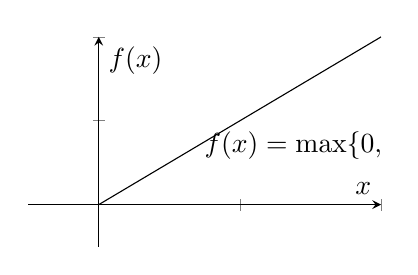
\begin{tikzpicture}
						\begin{axis}[
							xlabel = $x$,
							ylabel = {$f(x)$},
							xmin = -.5, xmax = 2,
							ymin = -.5, ymax = 2,
							width = 0.5\textwidth,
							height = 0.35\textwidth,
							xticklabel = \empty,
							yticklabel = \empty,
							axis lines = middle,
							domain = -.5:2,
							samples = 100,
							]
							\addplot[black, domain = 0:2] {x};
							\node at (axis cs: 1.5, .7) {$f(x) = \max\{0, x\}$};
						\end{axis}
					\end{tikzpicture}
					\caption{Función ReLU}
					\label{fig:funcion_relu}
				\end{figure}
				
				La función \gls{relu} es una de las más populares al trabajar con redes neuronales, pues a pesar de que no es derivable en $x = 0$ (normalmente se soluciona tomando $f'(0) = 1$), soluciona un serio problema que causan las funciones logística y tangente hiperbólica durante el entrenamiento de una red neuronal. Este problema es conocido como \textit{vanishing gradient} y de forma resumida consiste en que cuando la derivada de una función de activación es muy próxima a cero, relentiza enormemente el proceso de aprendizaje, pues si se observa con detalle cómo se calculan las actualizaciones de los pesos y sesgos en el \Cref{algo:backprop}, si los términos $\delta^{(s)}$ tienden a cero, la diferencia entre los parámetros de una iteración a otra tiende a cero, necesitando una cantidad enorme de iteraciones. Como se observa a continuación, la función \gls{relu} soluciona este problema. Además, la derivada es mucho más sencilla de calcular. 
				
				\begin{align*}
					\lim_{x\to\infty}\frac{d}{dx}\frac{1}{1+e^{-x}} = 0 && \lim_{x\to\infty}\frac{d}{dx}\tanh(x) = 0 && \lim_{x\to\infty}\frac{d}{dx}\text{ReLU}(x) = 1
				\end{align*}
				
				Si bien soluciona este problema mencionado para valores de $x > 0$, genera el mismo problema para valores negativos. Para solucionar este problema se suelen tomar variantes de la función \gls{relu} conocidas como LReLU, PReLU, o ELU; que modifican su expresión para valores de $x \leq 0$ como funciones lineales o exponenciales. 
				
				\item \textbf{Función softmax}\\
				
				Al abordar un problema de regresión con una red neuronal, puede entenderse como encontrar una función $\textbf{f}: \mathbb{R}^n \longrightarrow \mathbb{R}^m$, sin embargo, al utilizar redes neuronales para un problema de clasificación, lo que se necesita es una función $\textbf{f}: \mathbb{R}^n \longrightarrow [0, 1]^m$, es decir, se quiere obtener como respuesta el nombre de la clase a la que pertenece la entrada. La solución a este problema es introducir la función softmax en la capa de salida de la red. 
				
				$$
				\textbf{f}(\textbf{x}) = \frac{e^{\textbf{x}_i}}{\displaystyle\sum_{j = 1}^{k}e^{\textbf{x}_j}}
				$$
				
				Esta función verifica que $\sum_{p=1}^q \textbf{f}_p(\textbf{x}) = 1$, es decir, en la capa de salida de la red se obtiene la probabilidad de que una muestra presentada a la red pertenezca a una determinada clase. A dicha muestra se le asigna la clase que mayor probabilidad tiene. En este caso, no debe hablarse de su derivada sino de su matriz Jacobiana donde aparecerán las derivadas que puedan necesitarse durante \textit{Backpropagation}, siendo de la forma
				$$
				\frac{\partial \textbf{f}_i(\textbf{x})}{\partial \textbf{x}_j} = \textbf{f}_i(\textbf{x})(\delta_{ij} - \textbf{f}_j(\textbf{x})), 
				$$
				donde $\delta_{ij}$ es la función Delta de Kronecker. 
				
			\end{itemize}
			
		\section{Redes neuronales convolucionales}
		
			Una vez explicado cómo funciona una red neuronal y cómo puede usarse para problemas de regresión y clasificación, es interesante poder aplicar estas tareas sobre imágenes en vez de sobre conjuntos de datos numéricos. Una imagen de $n \times m$ píxeles en escala de grises puede entenderse como una matriz de $n \times m$ elementos, sin embargo, suelen utilizarse imágenes a color y esto se puede conseguir utilizando tres canales, rojo, azul, y verde. De esta forma, una imagen se representa como tres matrices. Formalmente, una imagen se representa como un tensor, que puede entenderse como un vector de matrices, o una estructura que indexa elementos mediante una tupla $(i, j, k)$.\\
			
			De manera ingenua, una primera aproximación para clasificar imágenes en función de objetos que aparezcan en estas, podría ser linealizar este tensor y pasarlo como vector de entrada a un red neuronal multicapa, obteniendo un vector de salida que indique a qué clase pertenece la imagen. Esto, además de que no da resultados positivos pues si se mueve o varía de tamaño el objeto a reconocer, la red ya no lo entendería igual al haber aprendido los valores de cada píxel concreto en cada caso; computacionalmente es muy complicado de abarcar. Suponiendo que se tiene una imagen \gls{rgb} cuadrada de $n \times n$ píxeles, y que la primera capa oculta tuviera $m$ neuronas, el número de parámetros de esta capa sería $m(3n^2 + 1)$. Suponiendo imágenes de baja calidad, por ejemplo $64 \times 64$ píxeles, y que el número de neuronas de la primera capa fuese 5, el número de parámetros es de 61445. Ajustar adecuadamente esa cantidad de parámetros muy costoso, y además daría resultados muy pobres en el caso de encontrar los parámetros adecuados. Se necesita simplificar la magnitud del problema y enseñar a la red a ver y entender, no solo aprender valores de píxeles. \\
			
			La forma de trabajar con imágenes y redes neuronales consiste en ``resumir'' las diferentes regiones de la imagen pasando como entrada de la red neuronal aquellas características destacables, es decir, un vector o mapa de características propias de la imagen. Un ejemplo de estos se muestra en la \Cref{fig:features}. Esto se puede lograr mediante las operaciones de convolución y correlación cruzada. 
			
			\begin{figure}[!h]
				\centering
				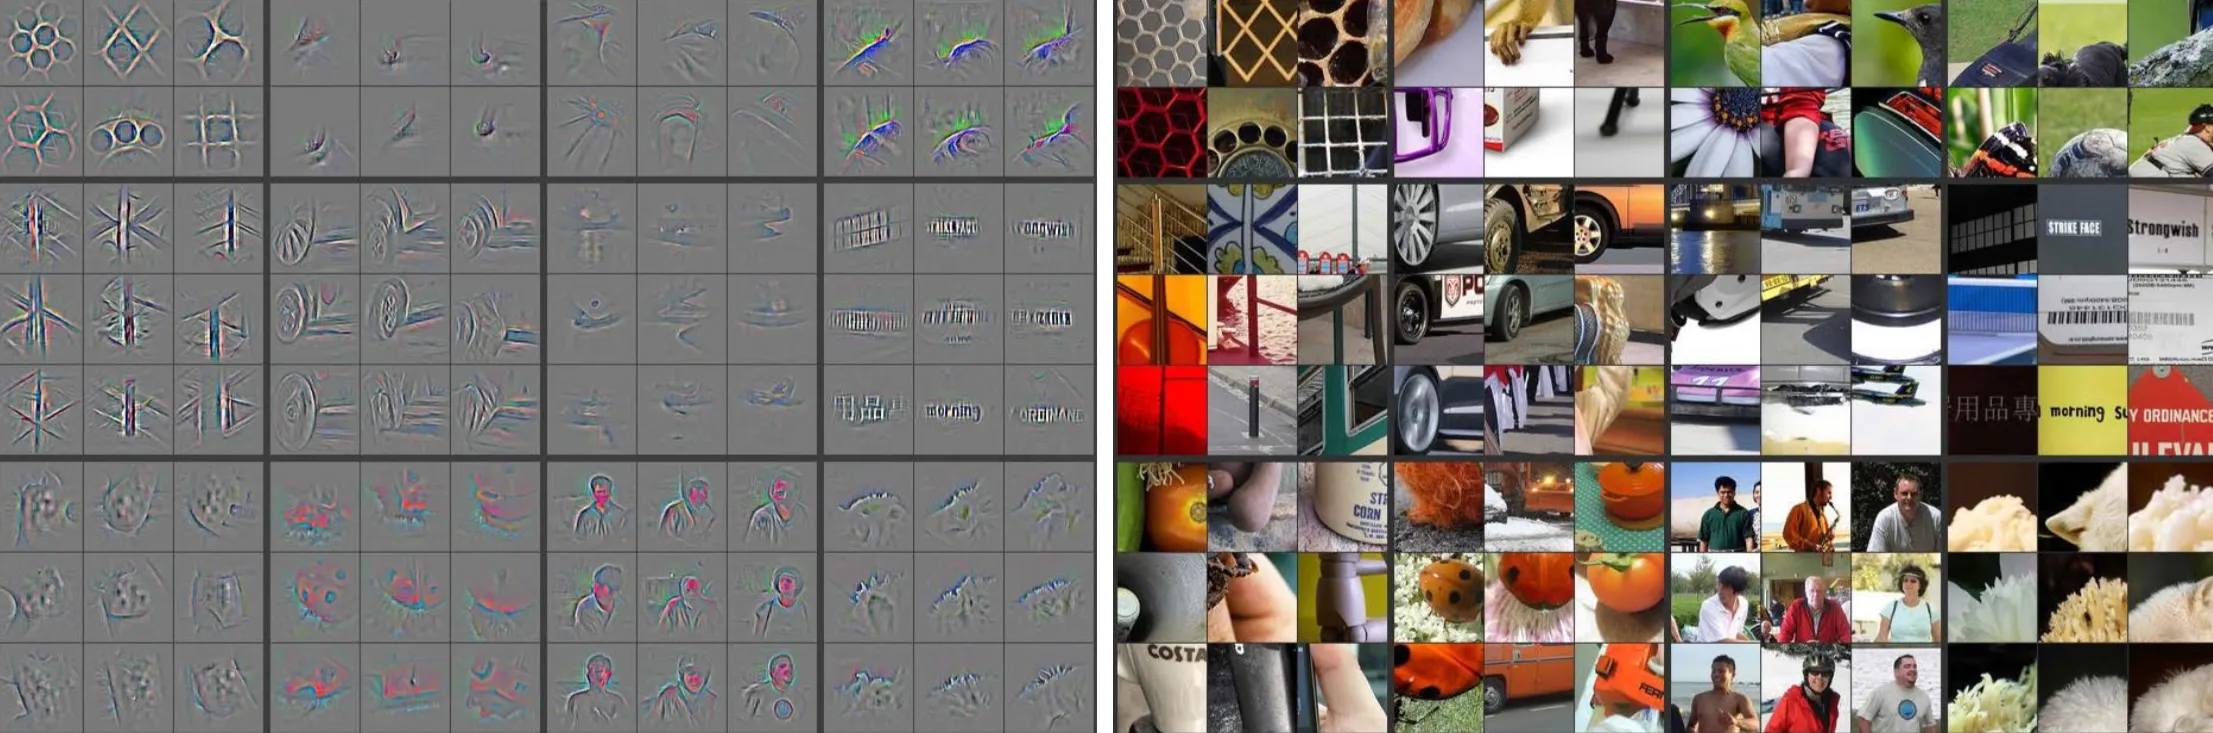
\includegraphics[scale = .2]{features}
				\caption{Imágenes y sus mapas de características \cite{features}}
				\label{fig:features}
			\end{figure}
			
			Una de las operaciones matemáticas más conocidas y que es más usada al trabajar con señales e imágenes es la llamada convolución, denotada por $\ast$, y dadas las funciones $f(t)$ y $g(t)$, su convolución se define de la siguiente manera. 
			
			$$
			(f \ast g)(t) = \int_{-\infty}^\infty f(\tau)g(t - \tau)\,d\tau
			$$
			
			En este caso se está asumiendo que el dominio de $f(\tau)g(t - \tau)$ es $\mathbb{R}$, lo que permite integrar sobre todo $\mathbb{R}$, de lo contrario, se modifica la definición para integrar solo sobre un intervalo $[a, b]$. En general, esta operación crea una nueva función a partir de otras dos, que indica cómo interactúan entre sí, y que permite aplicar filtros a señales e imágenes. Como se acaba de comentar para el caso de las imágenes, se puede tratar con señales que no dependan únicamente de una variable, pues estas se representan como una función de dos variables $f(u, v)$. En este caso, la convolución queda definida de la siguiente manera. 
			
			$$
			(f \ast g)(u, v) = \int_{-\infty}^\infty\int_{-\infty}^\infty f(\xi, \eta)g(u - \xi, v - \eta)\,d\xi\,d\eta
			$$
			
			Si bien en las definiciones previas se ha tomado la integral y tanto $\mathbb{R}$ como $\mathbb{R}^2$ como dominios continuos sobre los que calcular la convolución, no se debe olvidar que las imágenes no dejan de ser matrices o funciones de dos variables con un dominio discreto, por lo que se debe presentar una definición adecuada a este caso \cite{Goodfellow-et-al-2016}. 
			
			$$
			(f \ast g)(u, v) = \sum_{i=-k}^{k}\sum_{j=-k}^{k} g(i, j)f(u - i, v - j)
			$$
			
			En la expresión anterior, a la función $g(u, v)$ se le llama filtro o \textit{kernel} de convolución. A continuación se muestra un ejemplo de cómo calcular una convolución. 
			
			$$
			\begin{gathered}
				\begin{pmatrix}
					\tikzmarknode{a1}{1}& 2& 3& 4& 5\\ 
					5& 6& 7& 8& 9\\ 
					9& 8& \tikzmarknode{a2}{7}& 6& 5\\ 
					5& 4& 3& 2& 1\\
					1& 2& 3& 4& 5
				\end{pmatrix}
				\ast
				\begin{pmatrix}
					\tikzmarknode{b1}{1} & 0 & 0\\
					0 & 1 & 0\\
					0 & 0 & \tikzmarknode{b2}{1}
				\end{pmatrix}
				=
				\begin{pmatrix}
					\tikzmarknode{c1}{14} & 15 & 16\\
					16 & 15 & 14\\
					16 & 15 & 14
				\end{pmatrix}\\
				1 \cdot 1 + 2 \cdot 0 + 3 \cdot 0 + 5 \cdot 0 + 6 \cdot 1 + 7 \cdot 0 + 9 \cdot 0 + 8 \cdot 0 + 7 \cdot 1 = 14\\
				2 \cdot 1 + 3 \cdot 0 + 4 \cdot 0 + 6 \cdot 0 + 7 \cdot 1 + 8\cdot 0 + 8\cdot 0 + 7 \cdot 0 + 6 \cdot 1 = 15\\
				\vdots\\
				7 \cdot 1 + 6 \cdot 0 + 5 \cdot 0 + 3 \cdot 0 + 2 \cdot 1 + 1 \cdot 0 + 3 \cdot 0 + 4 \cdot 0 + 5 \cdot 1 = 14
			\end{gathered}
			\begin{tikzpicture}[remember picture, overlay]
				\draw ([shift={(-.5mm, .5mm)}]a1.north west) rectangle ([shift={(.5mm, -.5mm)}]a2.south east);
				\draw ([shift={(-.5mm, .5mm)}]b1.north west) rectangle ([shift={(.5mm, -.5mm)}]b2.south east);
				\path[->] ([shift={(-.5mm, .5mm)}]a1.north) edge [bend left = 15] ([shift={(-.5mm, 1mm)}]c1.north);
				\path[->] ([shift={(-.5mm, .5mm)}]b1.north) edge [bend left = 20] ([shift={(-.5mm, 1mm)}]c1.north);
			\end{tikzpicture}
			$$
			
			Aplicando diferentes kernels de convolución a una imagen se pueden extraer diferentes tipos de características de una imagen, como por ejemplo bordes. El filtro Sobel es capaz de hacer esto con los kernels que se muestran a continuación, pues se comportan como aproximaciones de las derivadas parciales de la imagen en un punto teniendo en cuenta los píxeles cercanos \cite{Gao2010}. 
			
			\begin{align*}
				G_u &= \frac{\partial f(u, v)}{\partial u} \approx \begin{pmatrix}
					-1 & 0 & 1\\
					-2 & 0 & 2\\
					-1 & 0 & 1
				\end{pmatrix}&
				G_v &= \frac{\partial f(u, v)}{\partial v} \approx \begin{pmatrix}
					-1 & -2 & -1\\
					0 & 0 & 0\\
					1 & 2 & 1
				\end{pmatrix}
			\end{align*}
			
			\begin{figure}[!h]
				\centering
				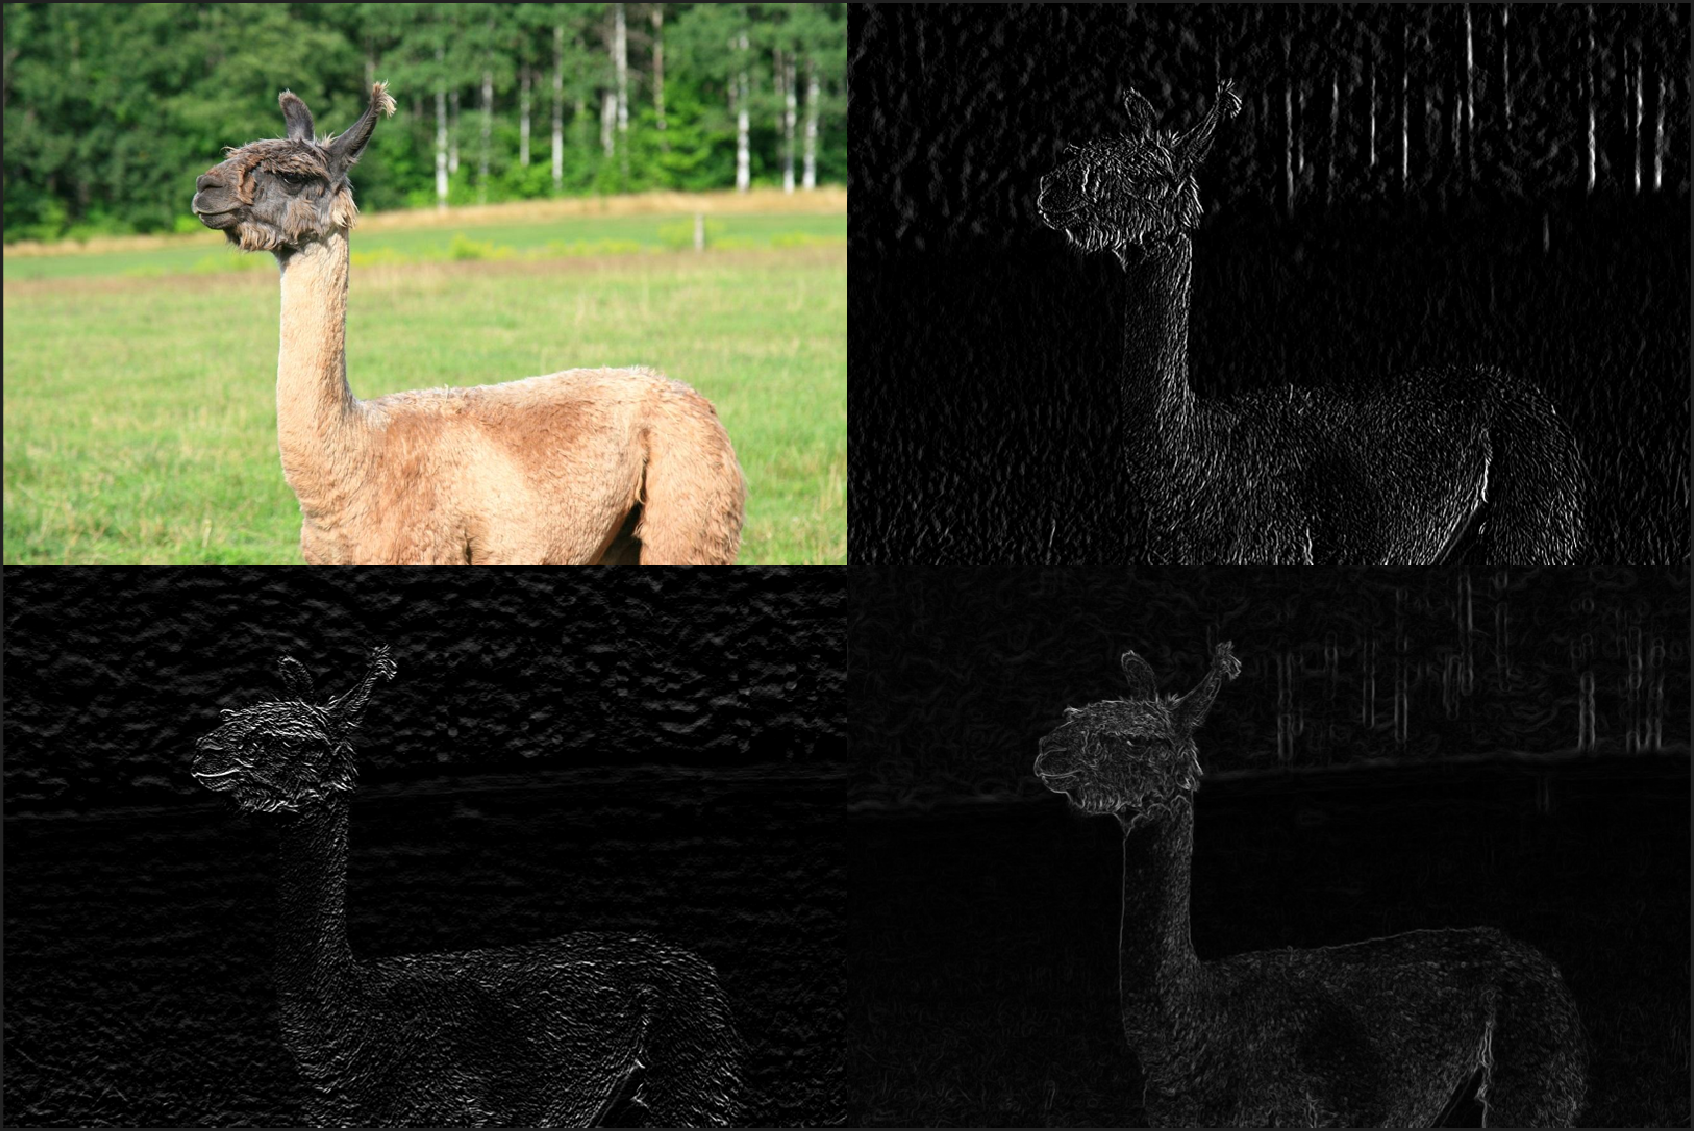
\includegraphics[scale = .4]{ejemplo_sobel}
				\caption{Detección de bordes aplicando los kernel Sobel}
				\label{fig:sobel}
			\end{figure}
			
			A continuación se va a calcular la convolución de la matriz del ejemplo anterior con $G_u$. Al realizar los cálculos como se ha mostrado en el ejemplo anterior, se obtiene como resultado la matriz $A$, mientras que al utilizar Python se obtiene la matriz $B$, los resultados no concuerdan. ¿Qué acaba de suceder? 
			
			\begin{align*} A &= 
				\begin{pmatrix}
					4 & 4 & 4\\
					-4 & -4 & -4\\
					-4 & -4 & -4
				\end{pmatrix}&
				B &= \begin{pmatrix}
					-4 & -4 & -4\\
					4 & 4 & 4\\
					4 & 4 & 4
				\end{pmatrix}
			\end{align*}
			
			La respuesta a estas preguntas se podría resumir en que se ha realizado una ``pequeña trampa'' a la hora de explicar cómo calcular la convolución manualmente en el ejemplo, ya que no se ha aplicado correctamente la definición dada. ¿Qué sentido tiene hacer esto? En visión artificial y tratamiento de imágenes, muchos autores y librerías llaman convolución a la operación que se ha mostrado en el primer ejemplo, cuando en realidad no lo es y trae lugar a confusión. Dicha operación se llama correlación cruzada, denotada por $(\star)$, y que es muy similar a la convolución, pues su principal diferencia es que en la convolución ``real'', el kernel se rota 180 grados antes de calcular la convolución ``falsa'' o correlación cruzada, es decir, $X \ast Y = X \star (R_{180} \cdot Y)$, donde $R_{180}$ es la matriz de rotación de 180 grados. En el primer ejemplo se ha utilizado de manera intencionada la matriz $I_3$ para ver los casos que traen lugar a confusión, pues $I_3 \cdot R_{180} = I_3$. La correlación cruzada de dos imágenes (matrices) se define de la siguiente manera \cite{Goodfellow-et-al-2016}. 
			
			$$
			(f \star g)(u, v) = \sum_{i=-k}^{k}\sum_{j=-k}^{k} g(i, j)f(u + i, v + j)
			$$
			
			Esta operación sí es con la que realmente se aplican los filtros a las imágenes y con la que se trabaja en general en el campo de la visión artificial. Es importante ver que ahora, al contrario que con la convolución, $f \star g \neq g \star f$. Algunas librerías de visión artificial tratan a la correlación cruzada como convolución debido al frecuente uso que tiene una sobre la otra y la forma similar que tienen de calcularse. Un ejemplo es OpenCV para Python y C++ en la documentación de su función \texttt{filter2D}, donde se comenta que aplica una convolución cuando realmente aplica la correlación cruzada \cite{OpenCVFiltering}. \\
			
			Finalmenete, a la hora de realizar estas operaciones, se pueden definir una serie de parámetros según convenga para obtener un tamaño diferente de salida \cite{introCNNformula}. Estos son \textit{stride} y \textit{padding}. El primero de ellos hace referencia a cada cuántos elementos se desplaza el kernel y se calcula el producto escalar, mientras que el segundo a cómo rellenar los bordes de la matriz original para obtener mayor tamaño de salida, habitualmente se colocan ceros en los bordes y se conoce como \textit{zero-padding}. El tamaño de salida se puede calcular como 
			$$
			\frac{n-k+2p}{s}+1, 
			$$
			y algunos valores por defecto para el \textit{padding} son \textit{valid},  \textit{full}, y \textit{same}. Con \textit{valid} no se añade ningún \textit{padding} de manera que el kernel solo se desliza en las zonas donde la matriz de entrada y el kernel coinciden por completo, con \textit{full} se añaden las filas y columnas de ceros necesarias para poder deslizar el kernel por cualquier zona en la que coincidan la matriz y el kernel, y con \textit{same} también se añaden las necesarias como para producir un tamaño de salida igual al de entrada. A partir de ahora, cuando se utilice el parámetro \textit{full}, las operaciones se escribirán como $\circledast$ y $\ostar$, pues la definición original se entiende como \textit{valid}. En ambos casos se tomará un \textit{stride} de 1. \\
			
			En general, para poder clasificar imágenes, se utilizan redes convolucionales por el motivo explicado, y para realizar dicha tarea se van concatenando diferentes tipos de capas, encontrándose entre estas las que se muestran a continuación \cite{introCNN}. Combinándolas se crea una red convolucional como por ejemplo, la que se muestra en la \Cref{fig:vgg16}, que se trata de la red VGG-16. \\
			
			\begin{figure}[!h]
				\centering
				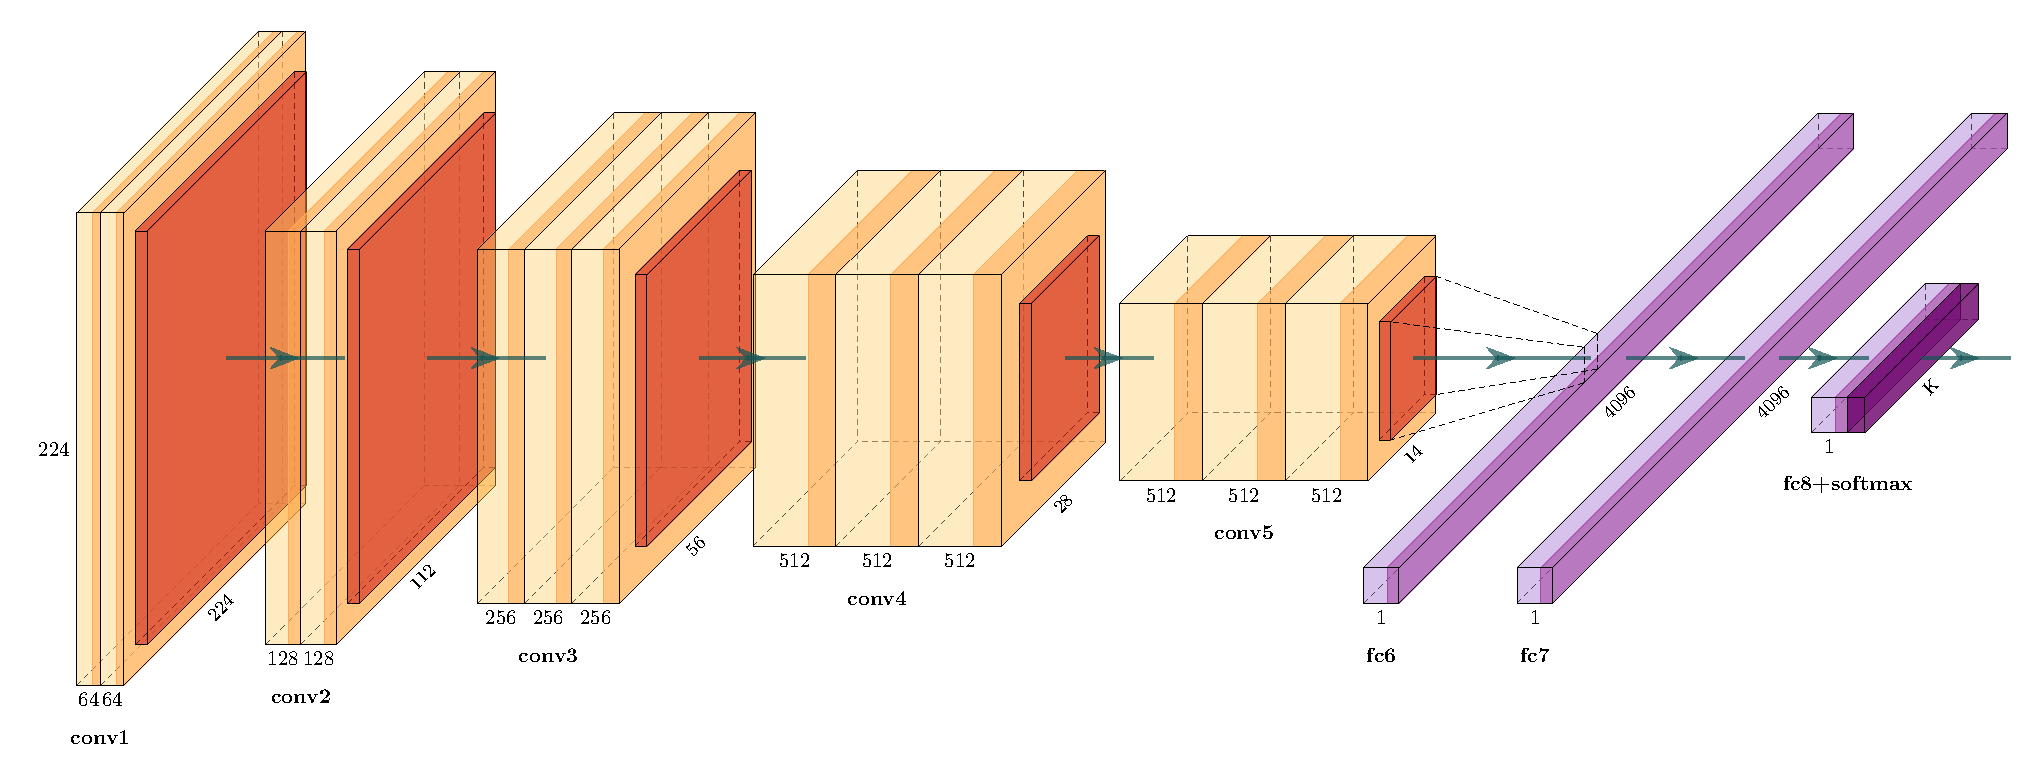
\includegraphics[width = \linewidth]{vgg16}
				\caption{Red convolucional VGG-16}
				\label{fig:vgg16}
			\end{figure}
			
			\begin{itemize}
				\item \textbf{Capa de entrada}\\
				Esta capa recibe la entrada de la red, normalmente la imagen representada como un tensor, es decir, una matriz por cada canal de la imagen. 
				
				\item \textbf{Capa de convolución}\\
				En este tipo de capas es donde reside principalmente el conocimiento de una red convolucional, pues dispone de unos parámetros llamados \textit{kernels} y \textit{bias}, o sesgos. Lo que hace esta capa es calcular la correlación cruzada entre la entrada y el kernel y sumar un sesgo, a pesar de que comúnmente se dice que calcula la convolución, como se ha discutido previamente. El número de salidas de esta capa depende del número de kernels y sesgos que se definan, se puede establecer un símil con el número de neuronas de una capa de una red neuronal. La entrada de la capa, que es un tensor, puede entenderse como una serie de matrices $X_i^{(m)}$, los kernels que serían otros tensores, como otra serie de matrices $K_{ij}^{(m)}$, y los sesgos como las matrices $B_i^{(m)}$, teniendo la siguiente ecuación para la salida de una capa de convolución. 
				
				$$
				N_i^{(m)} = B_i^{(m)} + \sum_{j = 1}^n X_j^{(m)} \star K_{ij}^{(m)}
				$$
				
				\item \textbf{Capa de activación}\\
				Al igual que en las redes neuronales clásicas se aplicaba una función de activación a la salida de cada neurona, en las redes convolucionales es habitual hacer esto mismo con las salidas de una capa de convolución y la función \gls{relu}. Se aplica esta a cada elemento del tensor de salida, pudiendo verse como sustituir por ceros aquellos valores negativos producidos por la correlación cruzada. 
				
				\item \textbf{Capa de \textit{pooling} o agrupación}\\
				Como previamente se ha mencionado, la ventaja de trabajar con redes convolucionales en vez de con las clásicas, es que estas son capaces de extraer las características importantes de una imagen, ``resumiendo'' esta antes de comenzar el trabajo de clasificación. Parte de este ``resumen'' se realiza mediante las capas de \textit{pooling} o agrupación. Se suelen utilizar las funciones maxpooling o avgpooling con kernels de tamaño $2\times2$ sobre la entrada, reduciendo el tamaño de esta en un 25\%. 
				
				$$
				\begin{gathered}
					f(x_1, x_2, \hdots, x_n) = \text{maxpooling}\{x_1, x_2, \hdots, x_n\} = \max\{x_1, x_2, \hdots, x_n\}\\
					\frac{\partial f}{\partial x_i} = \begin{cases}
						1 & \text{si } x_i = f(x_1, x_2, \hdots, x_n)\\
						0 & \text{si } x_i \neq f(x_1, x_2, \hdots, x_n)
					\end{cases}\\
					\text{maxpooling}\left(\begin{array}{cc|cc}
						1 & 2 & 3 & 4\\
						5 & \boxed{6} & 7 & \boxed{8}\\\hline
						9 & 10 & 11 & 12\\
						13 & \boxed{14} & 15 & \boxed{16}\\
					\end{array}\right) = \begin{pmatrix}
						6 & 8\\
						14 & 16
					\end{pmatrix}\\\\
					g(x_1, x_2, \hdots, x_n) = \text{avgpooling}\{x_1, x_2, \hdots, x_n\} = \frac{x_1 + x_2 + \hdots + x_n}{n}\\
					\frac{\partial g}{\partial x_i} = \frac{1}{n}\\
					\text{avgpooling}\left(\begin{array}{cc|cc}
						1 & 2 & 3 & 4\\
						5 & 6 & 7 & 8\\\hline
						9 & 10 & 11 & 12\\
						13 & 14 & 15 & 16\\
					\end{array}\right) = \begin{pmatrix}
						3.5 & 5.5\\
						11.5 & 13.5
					\end{pmatrix}
				\end{gathered}
				$$
				
				\item \textbf{Capa densa o totalmente conectada}\\
				Esta capa se trata de una de las capas de una red neuronal clásica. Recibe los vectores de características una vez han sido simplificados lo suficiente como para que una red clásica pueda trabajar con ellos y encontrar las relaciones entra las características de las imágenes de una misma clase. 
				
				\item \textbf{Capa softmax}\\
				Esta capa aplica la función softmax en la salida de la red neuronal para poder ajustar la salida a un problema de clasificación usual, tal y como se ha explicado anteriormente. 
			\end{itemize}
			
			Habiendo mostrado ya la arquitectura de una red convolucional con sus correspondientes parámetros (kernels y sesgos) e hiperparámetros (\textit{padding} y \textit{stride}), la pregunta clásica es, ¿cómo obtener los parámetros adecuados? La respuesta de cómo obtenerlos es simple, siendo algo más complicada de responder esta vez la de cuáles son. Al no dejar de ser una red neuronal, para obtener los parámetros de la red se utiliza \textit{Backpropagation} (\Cref{algo:backprop}) también, añadiendo las siguiente ecuaciones \cite{backpropCNN} al cálculo del gradiente para las capas de convolución. En este caso también aparece la recursividad mediante las sensibilidades de convolución $\Lambda_i^{(m)}$ hasta llegar a las sensibilidades clásicas $\delta_i^{(m)}$. 
			
			$$
			\begin{gathered}
				\Lambda_i^{(m)} = \frac{\partial L}{\partial N_i^{(m)}}\\
				\frac{\partial L}{\partial B_{i}^{(m)}} = \Lambda_i^{(m)}\\
				\frac{\partial L}{\partial K_{ij}^{(m)}} = X_j^{(m)}\star\Lambda_i^{(m)}\\
				\frac{\partial L}{\partial X_j^{(m)}} = \sum_{i = 1}^n\Lambda_i^{(m)}\circledast K_{ij}^{(m)}
			\end{gathered}
			$$
 		
			En este caso, como se comentaba anteriormente, a pesar de contar con el algoritmo para hallar los parámetros, no es suficiente para entrenar la red y obtener un resultado adecuado. Las redes convolucionales son un modelo de deep learing que necesita cantidades de datos y un poder computacional muy elevado. Para obtener un resultado decente se necesitan muchísimos datos de ejemplo y equipos con muchos recursos, como diferentes GPUs y grandes cantidades de memoria. 
			
		\section{Transformers}
			
			Si bien llegado este punto se podría afirmar que se ha conseguido una arquitectura que puede lograr el fin de este proyecto (clasificar imágenes), esta es mejorable en diversas situaciones. Supóngase que se dispone de un gran conjunto de imágenes de animales terrestres, acuáticos, y aéreos; y se necesita un modelo capaz de distinguir animales entre estas tres clases. Tras etiquetar estas imágenes manualmente, encontrar una arquitectura de \gls{cnn} adecuada, y entrenarla, se obtiene un clasificador capaz de distinguir entre estas tres clases. Tiempo más tarde, surge la necesidad de poder clasificar dentro de estas tres clases, por ejemplo, dentro de los animales acuáticos poder distinguir entre peces de río, ballenas, tiburones, etc. Esto supondría reetiquetar el dataset manualmente, modificar la arquitectura de las capas densas, y volver a entrenar el modelo. Considerando un caso extremo, podría además ser el dataset muy grande y no conocerse el número de especies dentro de cada una de las clases iniciales y querer separar las imágenes por cada una de las especies. Esto no sería posible con una \gls{cnn}, pues necesitaría tener definidas una serie de clases. \\
			
			Por otro lado, supóngase que dado un texto que describa una imagen, por ejemplo ``\textit{Un pastor alemán corriendo en un bosque}'', se quiere obtener la imagen del dataset que se adapta mejor a esa descripción, o se quiere obtener cómo de similares son dos imágenes del dataset, o se quiere extraer el texto que contiene una imagen, o se quiere comprobar cómo de bien se adapta una descripción de una imagen a esta. Todo este tipo de tareas y similares, serían imposibles de realizar mediante redes convolucionales, ya que no están enfocadas a trabajar con texto, y es aquí donde entran este tipo de modelos llamados transformers. Se presentaron en 2017 en un artículo escrito por investigadores de Google (con un nombre bastante acertado, \textit{Attention is all you need} \cite{attention}) como un modelo sustituto de las redes neuronales recurrentes debido al problema que tienen al intentar recordar información de instantes alejados. La idea original era utilizarlos para problemas de \gls{nlp}, como por ejemplo la traducción de textos, pero se pueden aplicar a una diversidad de problemas. Basándose en dicho artículo, se presenta una breve explicación de cómo funciona la arquitectura de un transformer. \\
			
			\begin{figure}[!h]
				\centering
				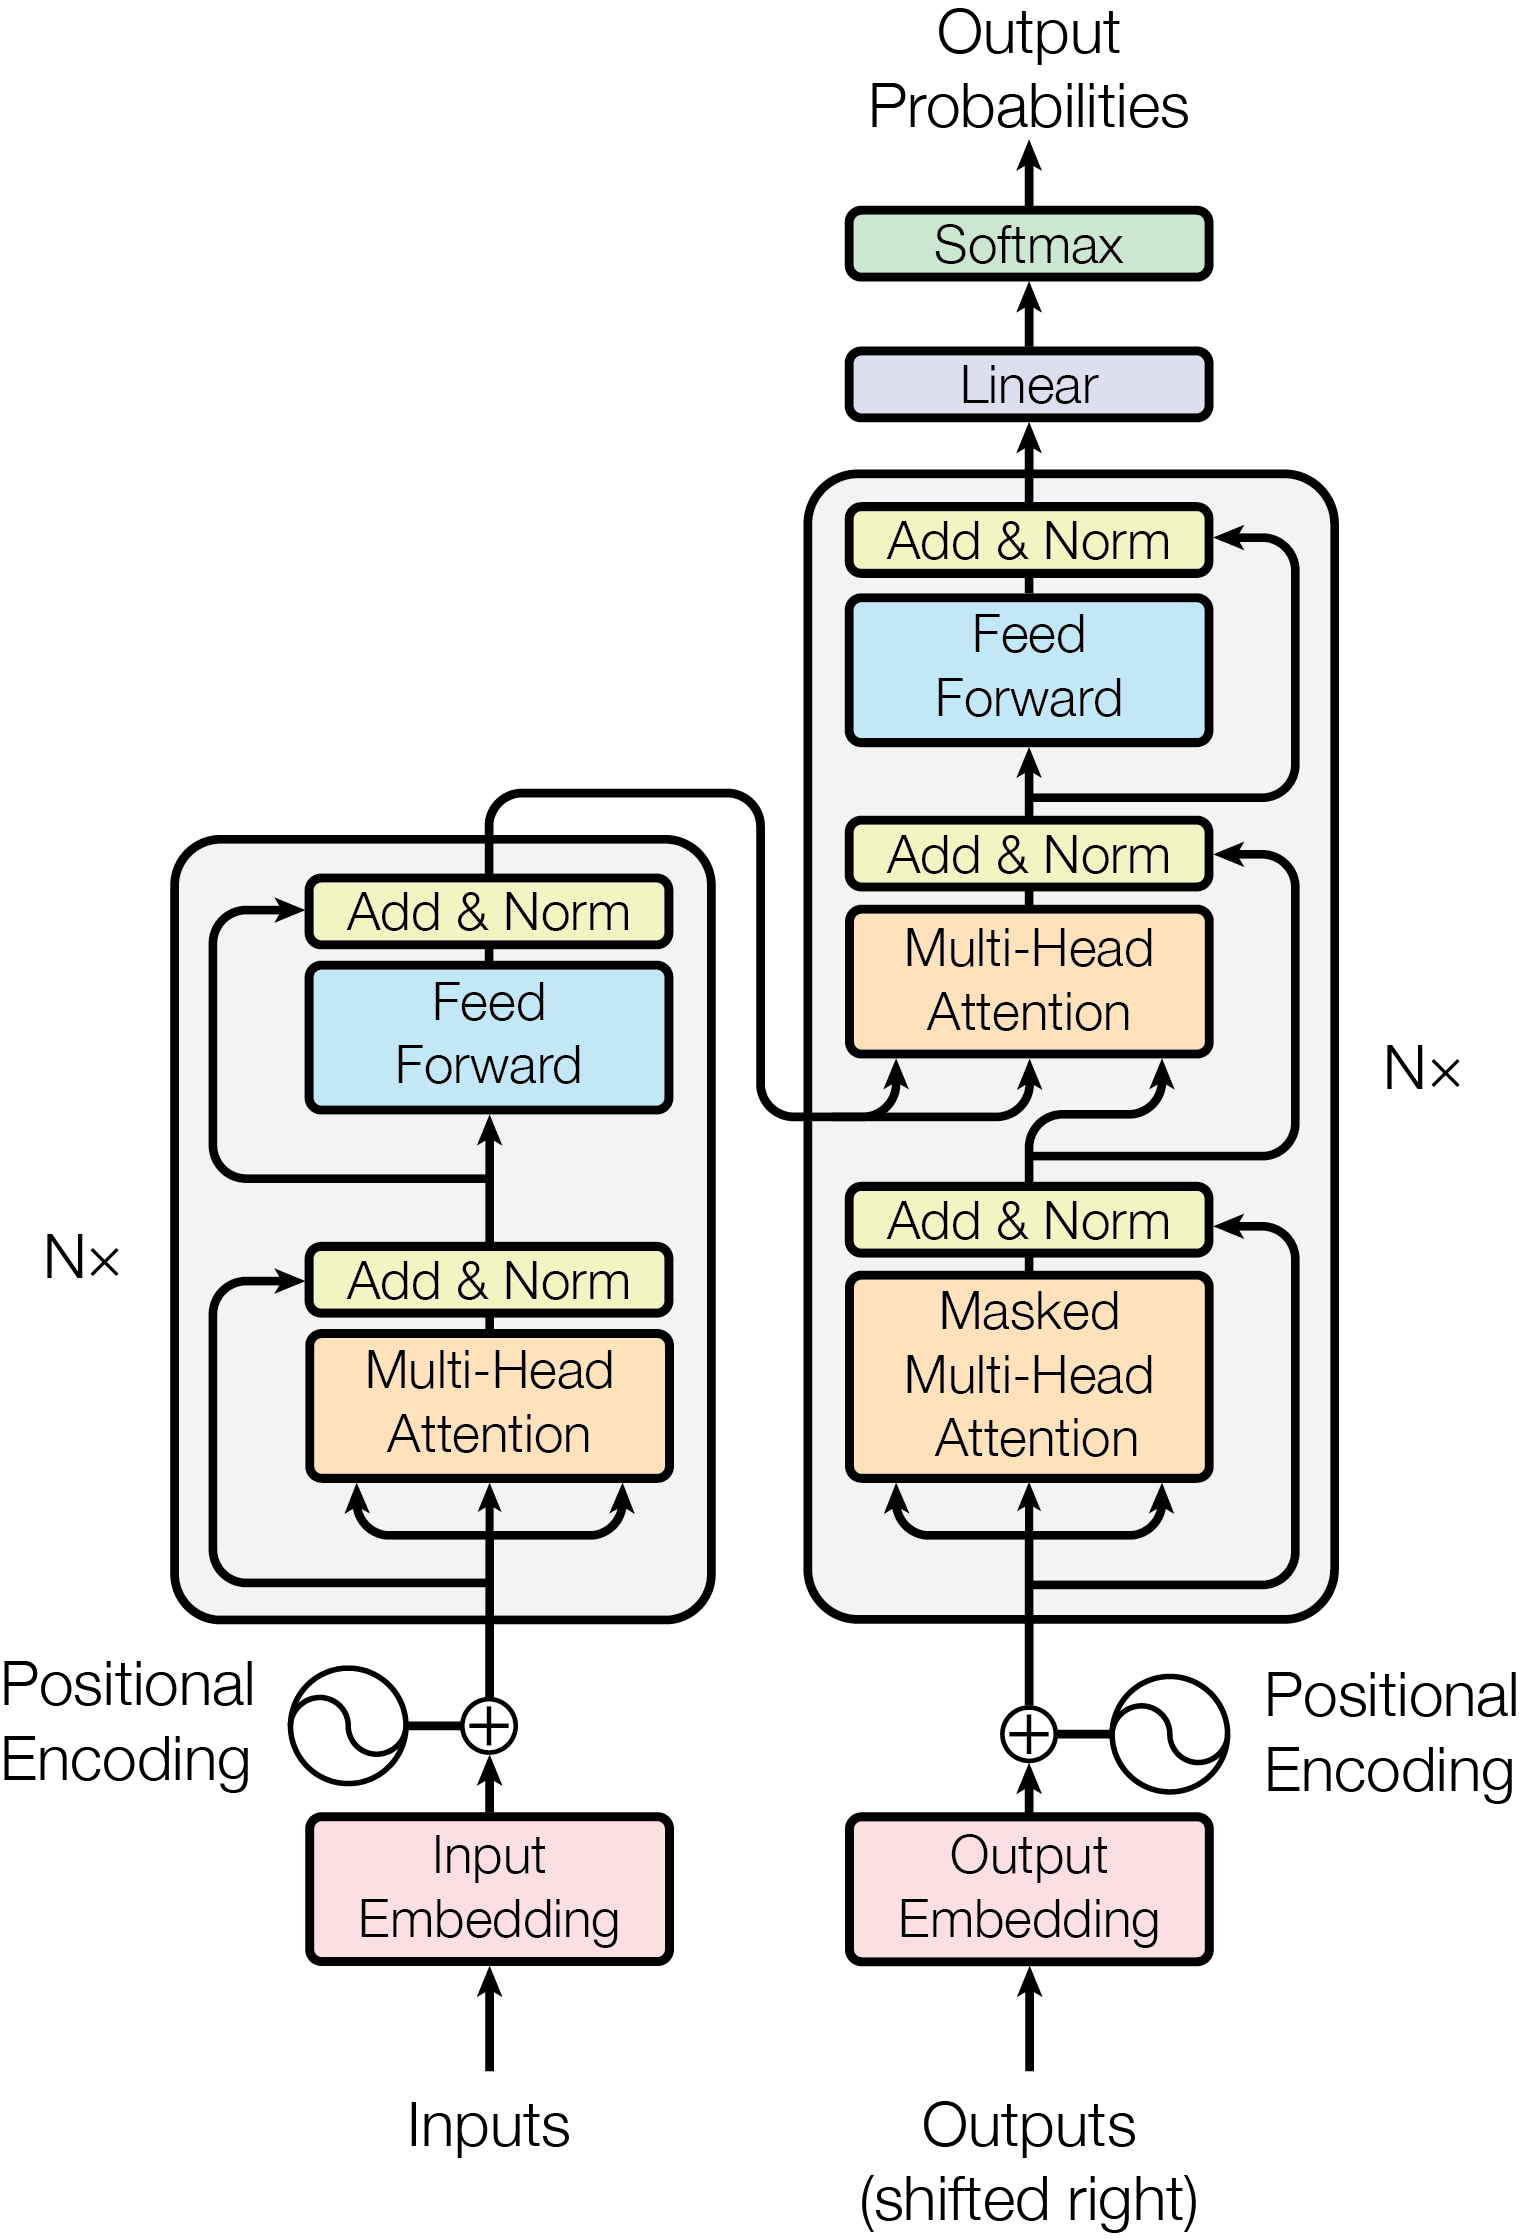
\includegraphics[scale = .5]{transformer}
				\caption{Arquitectura de un transformer codificador-decodificador \cite{attention}}
				\label{fig:arq_transf}
			\end{figure}
			
			\subsection{Codificación}
			
				El flujo que sigue un elemento de entrada en un transformer, es bastante más elaborado que el que se sigue en una red neuronal, tal y como se observa en la \Cref{fig:arq_transf}. Inicialmente comienza con la etapa de codificación, el la que el elemento recibido (en este primer ejemplo, un texto) se divide en una serie de tokens o elementos básicos e indivisibles, se añaden los tokens \texttt{\$SOS\$} (start of sequence) y \texttt{\$EOS\$} (end of sequence) para marcar el inicio y el final del contenido, y se convierte cada uno de ellos en una serie de embeddings $\textbf{e} \in \mathbb{R}^{d_m}$ que codifican el token. Un ejemplo sería dividir una frase por palabras, y asignar un vector diferente a cada palabra del diccionario, aunque en los modelos reales de \gls{nlp} no separan de esta manera. Continuando con el proceso, se necesita almacenar de alguna manera la posición de los tokens de entrada, pues el transformer procesa todos los tokens de manera simultánea y la frase ``\textit{Juan es mayor que María}'', es totalmente diferente a, por ejemplo ``\textit{María es mayor que Juan}'', a pesar de ser dos secuencias con los mismos tokens. Para lograr esto, a cada embedding \textbf{e} se le suma un vector posicional \textbf{p} donde cada una de sus componentes $p_i$ se obtienen de la siguiente manera, siendo $d_m$ la dimensión de los embeddings y $n$ la posición del token. 
				
				$$
				p_i(n) = \begin{cases}
					\text{sen}\left(\frac{n}{10000^{\frac{2i}{d}}}\right) & \text{si}\, i \equiv 0 \pmod{2}\\
					\cos\left(\frac{n}{10000^{\frac{2i}{d}}}\right) & \text{si}\, i \not\equiv 0 \pmod{2}\\
					\end{cases}
				$$
				
				Existen diferentes de maneras de codificar posiciones de tokens, pero en la arquitectura original se utilizó la presentada. El siguiente paso es el conocido como algoritmo de atención, siendo su misión la siguiente. Observando las frases ``\textit{Juan es un catador profesional de vino}'' y ``\textit{María vino ayer de Madrid}'', se ve que el token \texttt{vino} aparece en ambas, e inicialmente se le asignaría un embedding idéntico (excepto por la posición), ignorando el contexto en el que aparece el token y perdiendo su significado original. De la misma manera, en la frase ``\textit{Ellos son Juan y María, él es alto y ella es baja}'', necesitaría codificarse que los tokens \texttt{alto} y \texttt{baja} se refieren respectivamente a los tokens \texttt{él} y \texttt{ella}, y a su vez a los tokens \texttt{Juan} y \texttt{María}. La misión del algoritmo de atención es justo esta, transformar los embeddings de cada token para que su codificación se adapte al contexto. \\
				
				Esto se logra mediante tres matrices $Q$, $K$, y $V$ que se llaman query o consulta, key o clave, y value o valor, respectivamente. En este primer ejemplo, dichas matrices son copias de la matriz $E$ de embeddings. La idea es que cada embedding pregunte al resto cómo de relacionados están mediante $QK^T/\sqrt{d_m}$. Esto no es más que el producto escalar de cada par de embeddings normalizado, siendo una manera de medir la similitud entre dos vectores, que al aplicar la función softmax por filas, permite ver claramente para cada embedding cuál le ``presta más atención''. A veces, conviene aplicar una máscara $M$ con ciertos valores de $-\infty$ para forzar que algunos embeddings no presten atención a otros. El resultado obtenido se multiplica por la matriz de valores $V$. Esto representa que si un embedding está relacionado con otro, debe ``llevarse'' parte de él, para codificar tanto su información como la de aquellos embeddings con los que está relacionado. 
				
				$$
				A = \text{softmax}\left(\frac{QK^T\odot M}{\sqrt{d_m}}\right)V
				$$
				
				En este punto, se habría detectado la relación entre los tokens de \texttt{Juan} y \texttt{alto}, y los de \texttt{María} y \texttt{baja}, reflejando en la matriz $A$ el cambio que debe hacerse a cada embedding para que codifiquen la información del contexto recopilada. La matriz de embeddings, se actualizaría de manera que $E' = E + A$. Al realizar esta suma, el embedding del token \texttt{Juan} ya almacena información sobre que es alto. Este proceso se conoce como auto-atención ``de cabeza única'' o simple, pues normalmente se aplica el conocido como de ``cabeza múltiple''. \\
				
				\begin{figure}[!h]
					\centering
					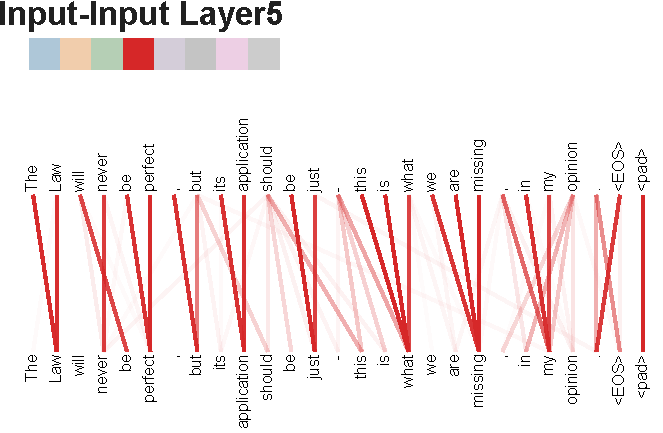
\includegraphics[scale = .7, angle = -90]{attention}
					\caption{Visualización del algoritmo de atención \cite{attention}}
					\label{fig:attention}
				\end{figure}
				
				\begin{algorithm}
					\SetProgSty{texttt}\DontPrintSemicolon
					
					\caption{Atención simple}
					\label{algo:attention_simple}
					
					\Datos{$E \in \mathbb{R}^{n \times d_m}, M \in \mathbb{R}^{n \times n}$}
					\Resultado{$E' \in \mathbb{R}^{n \times d_m}$}
					
					$A \gets \text{softmax}\left(\frac{QK^T\odot M}{\sqrt{d_m}}\right)V$\\
					$E' \gets E + A$
				\end{algorithm}
				
				La atención múltiple consiste en ejecutar en paralelo $h$ cabezas de atención.  Cada una cuenta con unas matrices $W_Q^{(i)}$, $W_K^{(i)}$, y $W_V^{(i)}$ de parámetros entrenables del modelo, que transforman el espacio de representación de los embeddings en $d_k = d_m / h$ para obtener $h$ matrices $A^{(i)}$. De esta manera, se consigue que cada cabeza aprenda los diferentes contextos que puede adoptar un token, para finalmente entre todas las cabezas, elegir el adecuado. Por ejemplo, en el caso del token \texttt{vino} esto ayuda a verificar si está actuando como verbo o como sustantivo. Para devolver los embeddings al espacio de representación original se utiliza una matriz $W_O$, también de parámetros entrenables. Esta variación se ve reflejada en el \Cref{algo:attention_multiple}. \\
				
				\begin{algorithm}
					\SetProgSty{texttt}\DontPrintSemicolon
					\SetKwBlock{Paralelo}{paralelamente hacer}{esperar}
					
					\caption{Atención múltiple}
					\label{algo:attention_multiple}
					
					\Datos{$E \in \mathbb{R}^{n \times d_m}, M \in \mathbb{R}^{n \times n}, W_Q^{(i)} \in \mathbb{R}^{d_k \times d_m}, W_K^{(i)} \in \mathbb{R}^{d_k \times d_m}, W_V^{(i)} \in \mathbb{R}^{d_v \times d_m}, W_O \in \mathbb{R}^{h d_v \times d_m}, h, 1 < i \leq h$}
					\Resultado{$E' \in \mathbb{R}^{n \times d_m}$}
					$d_k \gets \frac{d_m}{h}$\\
					$d_v \gets d_k$\\
					\Paralelo{
						$Q^{(i)} \gets E \left(W^{(i)}_Q\right)^T$\\
						$K^{(i)} \gets E \left(W^{(i)}_K\right)^T$\\
						$V^{(i)} \gets E \left(W^{(i)}_V\right)^T$\\
						$A^{(i)} \gets \text{softmax}\left(\frac{Q^{(i)}\left(K^{(i)}\right)^{t}\odot M}{\sqrt{d_k}}\right)V^{(i)}$
					}
					$E' \gets E + \left(A^{(1)}\middle|A^{(2)}\middle|\cdots\middle|A^{(h)}\right)W_O$
				\end{algorithm}
				
				El proceso de codificación continúa con una normalización de los embeddings. Para realizar dicha normalización \cite{normalization}, se supone que los elementos de cada embedding $\textbf{e}_i$ siguen una distribución $\mathcal{N}(\mu_i, \sigma_i)$, y se normalizan de acuerdo a la ecuación $E' = \Sigma\Gamma\odot(E - M) + B$, es decir, 
				\begin{align*}
					E' &= \begin{pmatrix}
						\sqrt{\sigma^2_1 + \varepsilon}^{-1} & 0 & \cdots & 0\\
						0 & \sqrt{\sigma^2_2 + \varepsilon}^{-1} & \cdots & 0\\
						\vdots & \vdots & \ddots & \vdots\\
						0 & 0 & \cdots & \sqrt{\sigma^2_n + \varepsilon}^{-1}\\
					\end{pmatrix}
					\begin{pmatrix}
						\gamma_{11} & \gamma_{12} & \cdots & \gamma_{1d_m}\\
						\gamma_{21} & \gamma_{22} & \cdots & \gamma_{2d_m}\\
						\vdots & \vdots & \ddots & \vdots\\
						\gamma_{n1} & \gamma_{n2} & \cdots & \gamma_{nd_m}\\
					\end{pmatrix} \\
					\odot&\quad \begin{pmatrix}
						e_{11} - \mu_1 & e_{12} - \mu_1 & \cdots & e_{1d_m} - \mu_1\\
						e_{21} - \mu_2 & e_{22} - \mu_2 & \cdots & e_{2d_m} - \mu_2\\
						\vdots & \vdots & \ddots & \vdots\\
						e_{n1} - \mu_n & e_{n2} - \mu_n & \cdots & e_{nd_m} - \mu_n\\
					\end{pmatrix} + \begin{pmatrix}
						\beta_{11} & \beta_{12} & \cdots & \beta_{1d_m}\\
						\beta_{21} & \beta_{22} & \cdots & \beta_{2d_m}\\
						\vdots & \vdots & \ddots & \vdots\\
						\beta_{n1} & \beta_{n2} & \cdots & \beta_{nd_m}\\
					\end{pmatrix}
				\end{align*}
				donde las matrices $\Gamma$ y $B$ son parámetros del modelo, y $\varepsilon$, ruido para evitar divisiones por cero. Se pretende que cada valor siga una distribución $\mathcal{N}(0, 1)$, quedando multiplicado y sumado por los parámetros de ganancia y sesgo. Para finalizar la etapa de la codificación, cada embedding normalizado pasa por una red neuronal clásica y se vuelve a normalizar la suma de la entrada y la salida de la red. 
				
			\subsection{Decodificación}
			
				La etapa de decodificación es bastante similar a la de codificación, ya que la misión del decodificador se puede resumir de manera informal en mezclar las codificaciones del codificador, y las codificaciones de la entrada del decodificador. Todos los bloques del decodificador que se muestran en la \Cref{fig:arq_transf} ya han sido explicados a excepción de un detalle. \\
				
				Aparece una capa de atención múltiple que es algo diferente de la comentada, ya que en realidad está calculando la atención múltiple-cruzada (\Cref{algo:attention_multiple-cruzada}). Este cálculo es idéntico al de la atención múltiple, pero en vez de utilizar los embeddings del decodificador ($E_2$) para calcular las consultas, claves, y valores; se utilizan solo para calcular las consultas. Para calcular las claves y valores se utilizan los embeddings de la salida del codificador ($E_1$), pues de esta manera ``preguntan'' a los del decodificador para encontrar las relaciones entre los tokens de entrada del codificador y los del decodificador. 
				
				\begin{algorithm}
					\SetProgSty{texttt}\DontPrintSemicolon
					\SetKwBlock{Paralelo}{paralelamente hacer}{esperar}
					
					\caption{Atención múltiple-cruzada}
					\label{algo:attention_multiple-cruzada}
					
					\Datos{$E_1 \in \mathbb{R}^{n \times d_m}, E_2 \in \mathbb{R}^{n \times d_m}, M \in \mathbb{R}^{n \times n}, W_Q^{(i)} \in \mathbb{R}^{d_k \times d_m}, W_K^{(i)} \in \mathbb{R}^{d_k \times d_m}, W_V^{(i)} \in \mathbb{R}^{d_v \times d_m}, W_O \in \mathbb{R}^{h d_v \times d_m}, h, 1 < i \leq h$}
					\Resultado{$E_2' \in \mathbb{R}^{n \times d_m}$}
					$d_k \gets \frac{d_m}{h}$\\
					$d_v \gets d_k$\\
					\Paralelo{
						$Q^{(i)} \gets E_2 \left(W^{(i)}_Q\right)^T$\\
						$K^{(i)} \gets E_1 \left(W^{(i)}_K\right)^T$\\
						$V^{(i)} \gets E_1 \left(W^{(i)}_V\right)^T$\\
						$A^{(i)} \gets \text{softmax}\left(\frac{Q^{(i)}\left(K^{(i)}\right)^{t}\odot M}{\sqrt{d_k}}\right)V^{(i)}$
					}
					$E_2' \gets E_2 + \left(A^{(1)}\middle|A^{(2)}\middle|\cdots\middle|A^{(h)}\right)W_O$
				\end{algorithm}
				
			\subsection{Ejecución y entrenamiento}
			
				Esta arquitectura fue planteada originalmente para lograr la traducción de textos de un idioma a otro, aunque como se comentará más adelante, es aplicable a diversas tareas. Suponiendo que se quiere traducir el texto ``\textit{Juan es alto}'', el flujo de ejecución es el siguiente. 
				\begin{enumerate}[label = \textbf{\arabic*. }]
					\item Se obtienen los tokens \texttt{\$SOS\$}, \texttt{Juan}, \texttt{es}, \texttt{alto}, \texttt{\$EOS\$}
					\item El codificador genera una matriz $E_1 \in \mathbb{R}^{5 \times d_m}$ y se envía al decodificador. 
					\item En la entrada del decodificador se introduce el token \texttt{\$SOS\$}, y a la salida deberían aparecen los tokens \texttt{\$SOS\$}, \texttt{John}. 
					\item En la entrada del decodificador se introducen los tokens generados por el propio decodificador \texttt{\$SOS\$} y \texttt{John}, y a la salida deberían aparecen los tokens \texttt{\$SOS\$}, \texttt{John}, \texttt{is}.
					\item Se continúa introduciendo la salida del decodificador en su entrada, hasta obtener en la salida el token \texttt{\$EOS\$}.
				\end{enumerate}
				
				Actualmente, los transformers pueden tener o no codificador y decodificador, clasificándose principalmente en función de esto. 
				\begin{itemize}
					\item Transformers con codificador y decodificador, normalmente orientados y originalmente diseñados para tareas de traducción. Un ejemplo es T5 de Google. 
					\item Transformers con sólo codificador, normalmente orientados a tareas de clasificación. Un ejemplo son los \gls{vit}. 
					\item Transformers con sólo decodificador, normalmente orientados a tareas de generación de contenido. Un ejemplo es GPT-4 de OpenAI. 
				\end{itemize}
				
				Respecto al entrenamiento, se utilizan las mismas técnicas que en las secciones anteriores, Backpropagation con las funciones de error y optimizadores adecuados, normalmente entropía cruzada y Adam, pues se quiere comparar el token esperado con el predicho. El motivo de utilizar Backpropagation es que un transformer no deja de ser una sucesión de redes neuronales. Por otro lado, añadir que para cada ejemplo de traducción se obtienen diferentes ejemplos con los que entrenar, pues para predecir el token $i$, se necesita predecir correctamente el token $i-1$, por lo que la predicción hasta cada token sirve como un ejemplo de entrenamiento diferente, lo que permite tener una gran cantidad de ejemplos. 
				
		\section{Transformers de visión}
		
			En la sección anterior se presentaban los transformers como un modelo capaz de mejorar el resultado que se puede obtener con redes convolucionales, además de añadir la capacidad de poder trabajar con texto. Hasta este momento se ha demostrado cómo mediante la arquitectura y algoritmos descritos son capaces de trabajar con textos, siendo ahora las principales preguntas, ¿cómo puede un transformer procesar una imagen? ¿Será necesario variar su arquitectura?\\
			
			En 2021, Google vuelve a publicar otro artículo \cite{vit} sobre transformers, donde plantean la posibilidad de utilizar este tipo de modelo en tareas relacionadas con imágenes al haber obtenido resultados tan positivos con textos. Al igual que en el artículo donde se presentaban los transformers por primera vez, este también cuenta con un título que resume la solución al problema para presentar los transformers de visión o \gls{vit}: ``\textit{Una imagen son $16 \times 16$ palabras}''. \\
			
			\begin{figure}[!h]
				\centering
				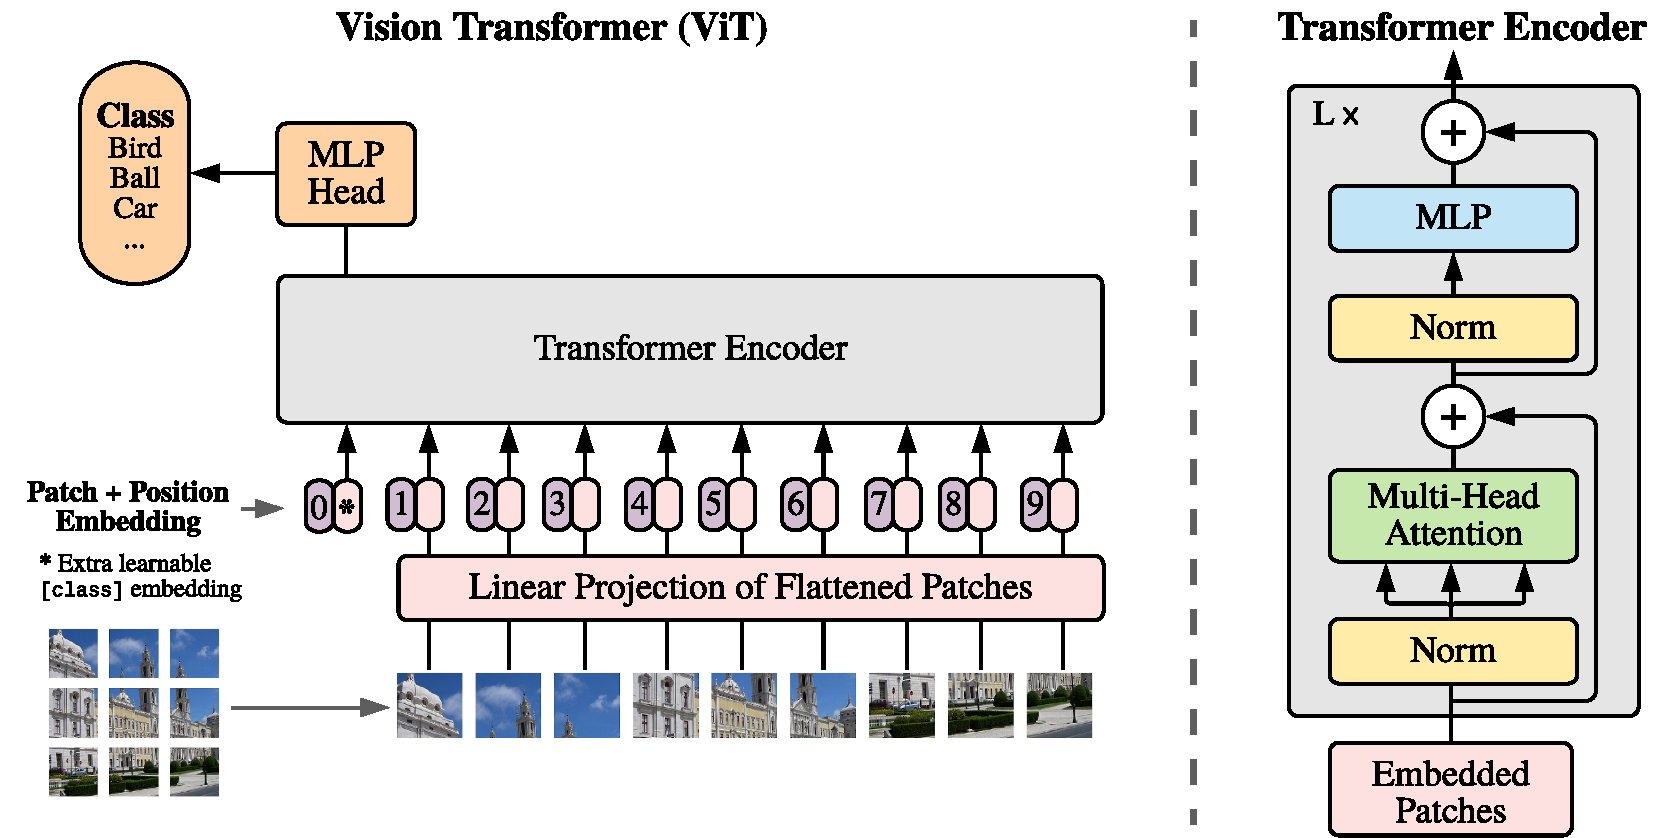
\includegraphics[scale = .5]{vit}
				\caption{Arquitectura de un transformer de visión \cite{vit}}
				\label{fig:vit_arq}
			\end{figure}
			
			En dicho artículo, se propone reutilizar lo máximo posible la arquitectura original del transformer. La primera de las diferencias reside en la entrada del modelo, y para ello se toma que una imagen consiste en un elemento de dimensiones ${h \times w \times c}$ y se propone separarlo en $n$ subimágenes $p^2 \times c$. Esto es análogo a separar un texto en palabras, excepto que en este caso, todos las divisiones tienen el mismo tamaño. De aquí proviene el nombre del artículo, ya que se propone dividir las imágenes originales en subimágenes de $16 \times 16$ píxeles. De esta manera se obtienen tokens de longitud $cp^2$, pero el modelo trabaja con embeddings de tamaño $d_m$, que mediante una serie de parámetros entrenables se realiza esta conversión de dimensiones. \\
			
			Al igual que en el transformer clásico, se necesita guardar información sobre la ubicación de cada subimagen. Aquí aparece la siguiente diferencia, pues cada elemento se ubica mediante una fila y columna, surgiendo el debate sobre si es necesario codificar las filas y columnas, o si basta con almacenar la posición de forma linealizada. Tras varios ensayos, se demuestra que a penas existen diferencias en los resultados obtenidos. \\
			
			La siguiente de las diferencias reside en el número de embeddings con los que trabaja un \gls{vit}. En el transformer clásico si se contaba con $n$ tokens, entonces la matriz de embeddings tenía dimensiones $n \times d_m$, mientras que con un \gls{vit}, es de $(n + 1) \times d_m$. Los transformers de visión trabajan con un token adicional comúnmente llamado \gls{cls}, que codifica información del resto de embeddings, es decir, codifica información de la imagen. Este vector permite la clasificación de las imágenes, pues con un \gls{vit} debidamente entrenado si recibe dos imágenes con cierta relación, entonces sus \gls{cls} deberían ser similares. En general, la salida de este modelo es este vector, para después, utilizarlo como la entrada de una red neuronal para poder clasificarlo. Aquí se observa que los \gls{vit} solo constan de la parte del codificador. 
			
		\section{Transformers multimodales}\label{sec:transformers_multimodales}
		
			En las secciones anteriores se ha demostrado cómo es posible la codificación y clasificación de texto e imágenes (en el caso de texto también generación), hasta el momento sin aparente mejora frente a los tipos de redes neuronales presentadas, pues no se ha respondido la cuestión de cómo trabajar con imágenes y textos simultáneamente, cómo modificar la clasificación de las imágenes o textos sin modificar la arquitectura (una red neuronal clásica clasifica en función del \gls{cls}), cómo realizar la clasificación sin conocer el número de clases, cómo realizar la clasificación sin contar con un dataset etiquetado, y una larga lista de tareas aparentemente complicadas y sin relación entre sí pero que tienen una solución común, los transformers multimodales. \\
			
			Los modelos multimodales son un tipo de modelos que permiten la entrada de información de diferentes fuentes en diferentes modalidades como por ejemplo, texto, audio, imágenes, vídeo, etc; y que son capaces de establecer relaciones entre estas \cite{multimodal_dl}. Desde el artículo que presentaba el modelo del transformer, cada vez son más las variantes de su arquitectura que aparecen para poder trabajar con diferentes tipos de datos, llegando en la actualidad hasta los transformers multimodales. Los más populares y que ayudan a responder las preguntas que se planteaban a lo largo de este trabajo, son aquellos capaces de trabajar con imágenes y textos. \\
			
			El objetivo principal de este tipo de transformers es ser capaz de representar los embeddings de texto y los de imágenes en un espacio común, de manera que por ejemplo los tres elementos mostrados en la \Cref{fig:info_multi}, tengan un embedding similar al tratar de representar un mismo concepto \cite{multimodal_transformers}.
			
			\begin{figure}[!h]
				\centering
				\begin{subfigure}{.3\textwidth}
					\centering
					
\includegraphics[scale = .35, valign = c]{imagen_texto_gato}
					\caption{Imagen de la palabra gato}
				\end{subfigure}\hfill
				\begin{subfigure}{.3\textwidth}
					\centering
					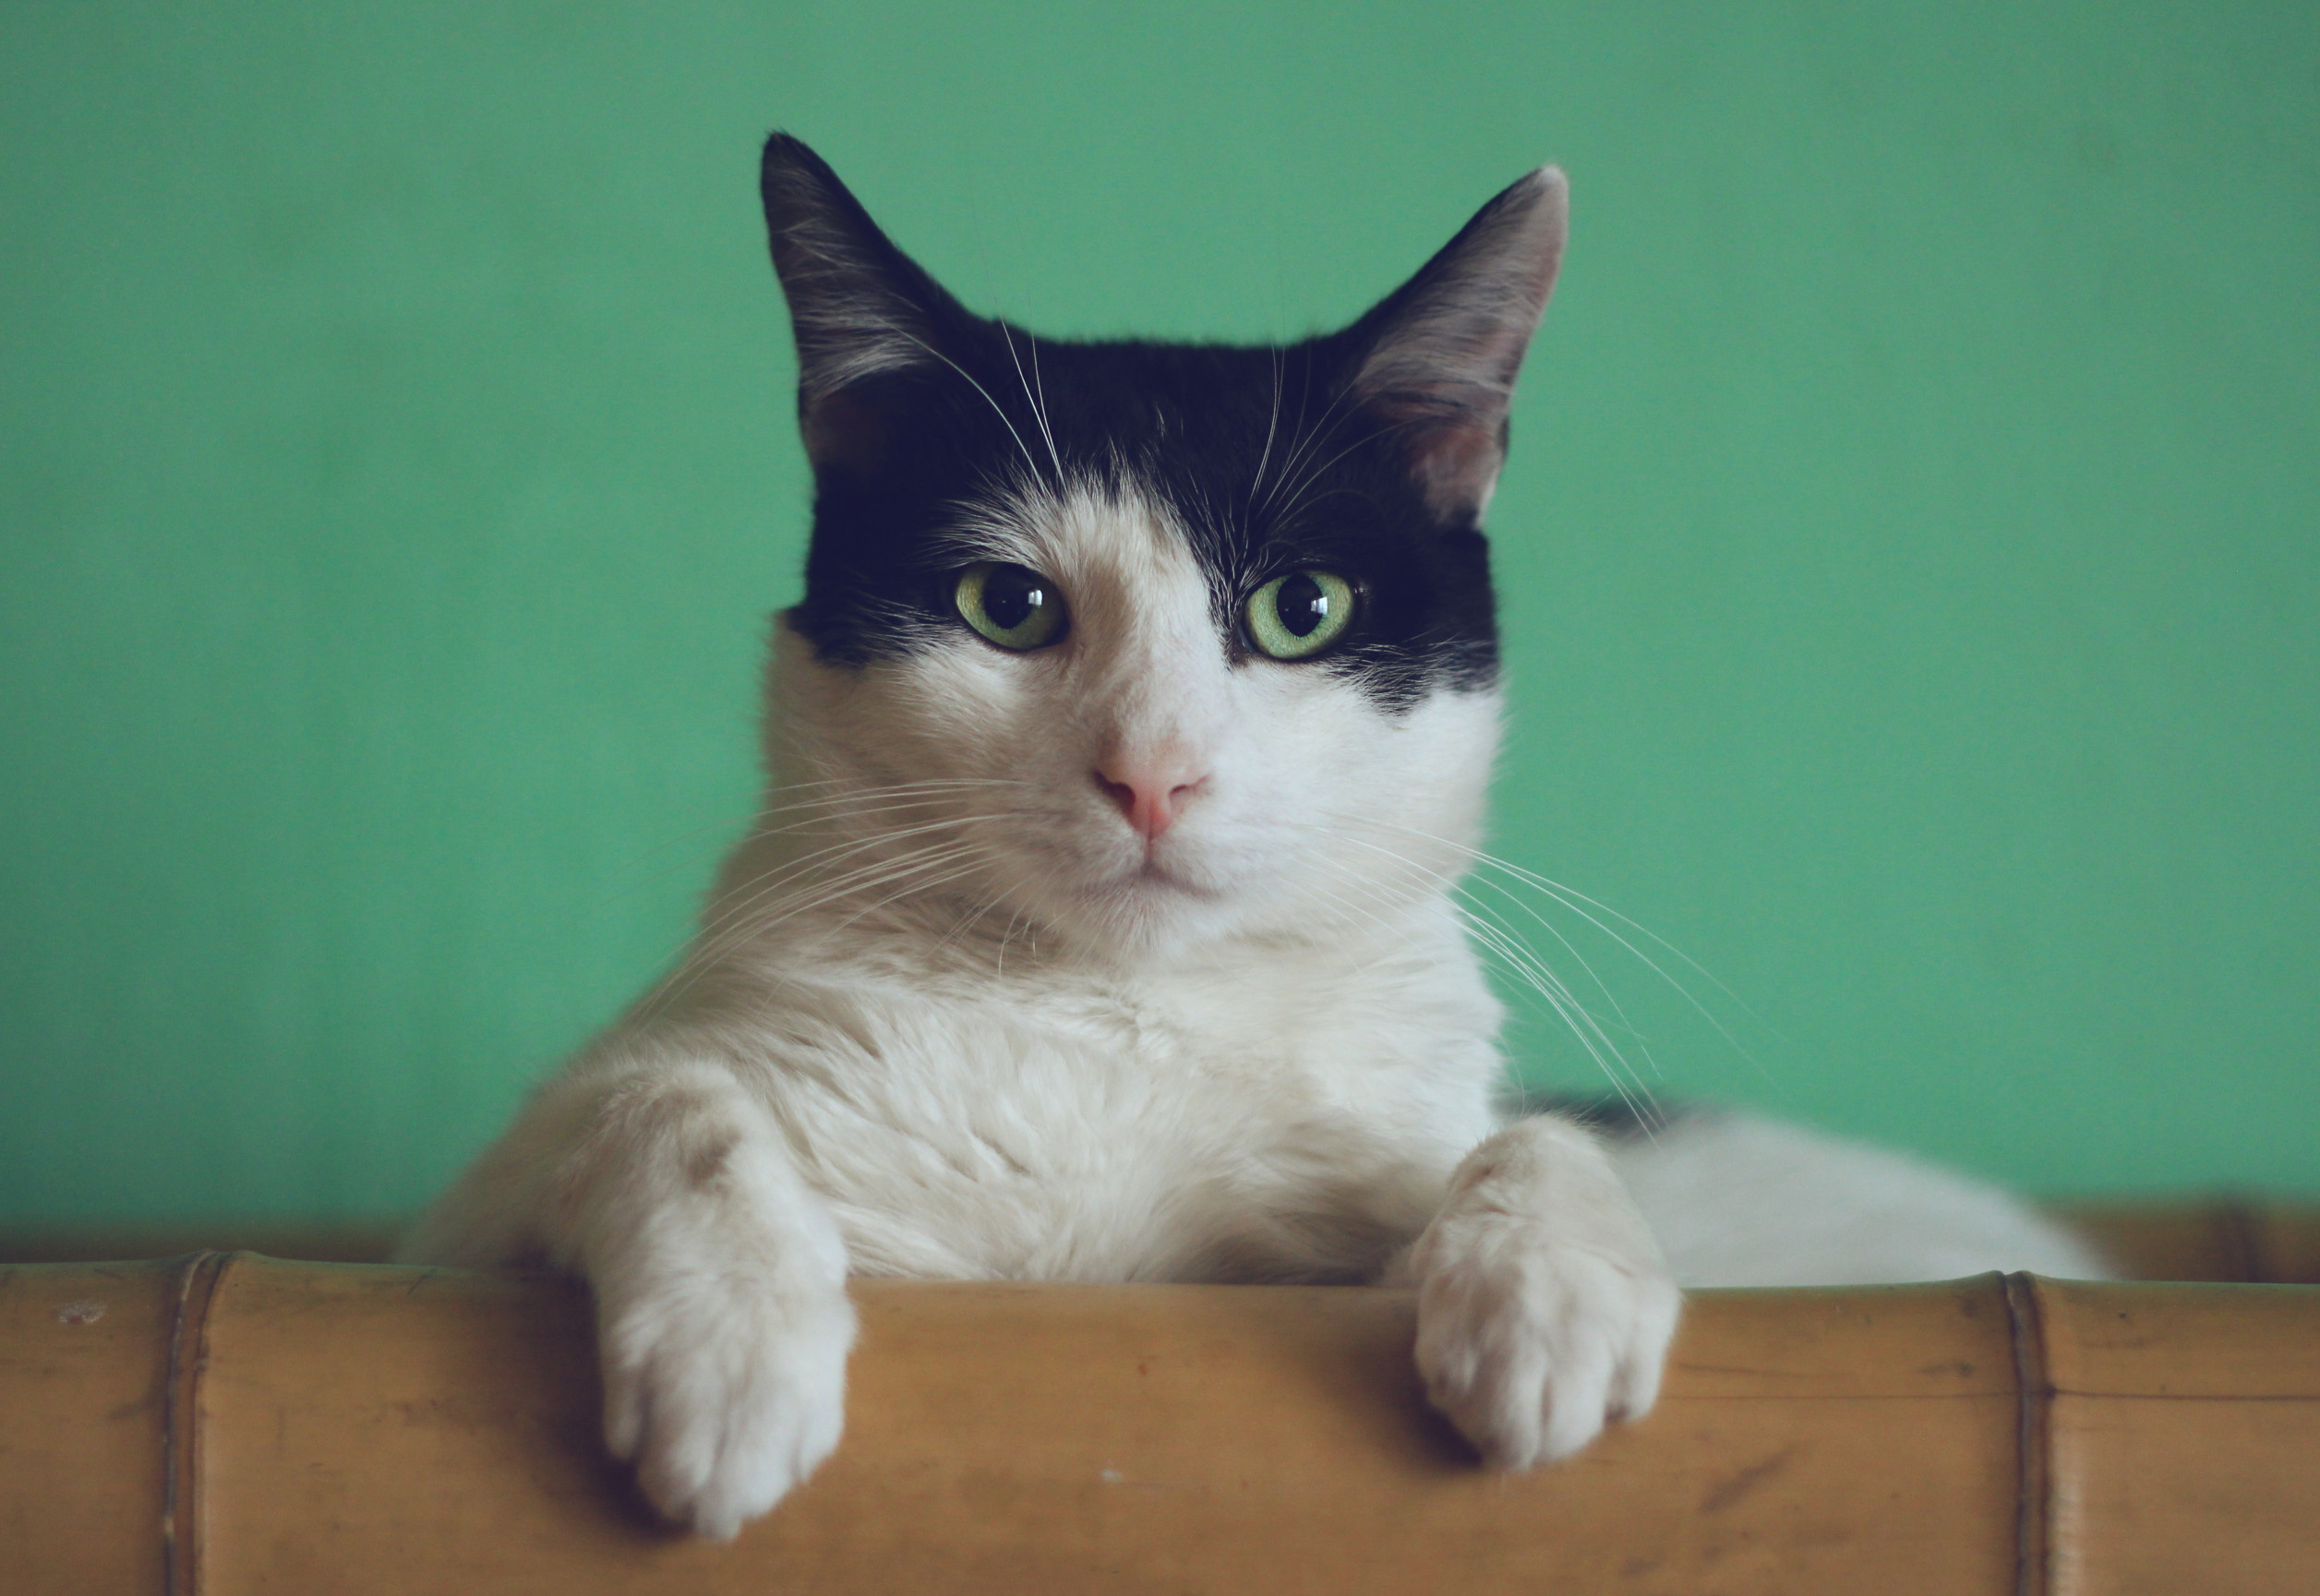
\includegraphics[scale = .05, valign = c]{imagen_gato}
					\caption{Imagen de un gato}
				\end{subfigure}
				\begin{subfigure}{.3\textwidth}
					\begin{minipage}[position][2.5cm][c]{\textwidth}
						\centering
						\Large\texttt{Cat}
					\end{minipage}
					\caption{Texto con la palabra gato}
				\end{subfigure}
				\caption{Información multimodal \cite{vertex}}
				\label{fig:info_multi}
			\end{figure} 
			
			Una manera de comparar si dos embeddings son similares es mediante el coseno del ángulo que forman ambos embeddings \cite{cosine}, pues no dejan ser vectores. Si el valor es próximo a uno significa que están codificando un concepto semánticamente relacionado al tener una dirección similar. Si el valor es próximo a cero, codifican ideas distintas, pues son dos vectores ortogonales, sus direcciones no son similares. En el caso de la \Cref{fig:info_multi}, si el transformer ha sido entrenado adecuadamente, el coseno formado por cada una de las tres posibles parejas de vectores debería ser similar y cercano a 1, indicando que las tres representaciones se refieren al mismo concepto. 
			
			$$
			\cos(\theta) = \frac{\textbf{a} \cdot \textbf{b}}{\|\textbf{a}\|\cdot\|\textbf{b}\|}
			$$
			
			Gracias a esta idea de tener conceptos en diferentes modalidades representados en un mismo espacio, se pueden realizar tareas muy útiles como la búsqueda de una imagen dada una descripción textual, la búsqueda de la imagen más similar a otra, la búsqueda del texto más similar a otro, etc. Todos estos problemas son en realidad el mismo, pues todos los elementos quedan representados como un vector y basta con comparar los cosenos entre cada par de embeddings, y elegir el mayor de todos, eligiendo así el embedding que tiene una dirección más similar a la dada. En la \Cref{fig:textos_imagenes} se visualiza cómo mediante esta idea es posible asignar a cada una de las $n$ imágenes, un conjunto de $k$ descripciones, donde $n \geq k$. 
			
			\begin{figure}[!h]
				\centering
				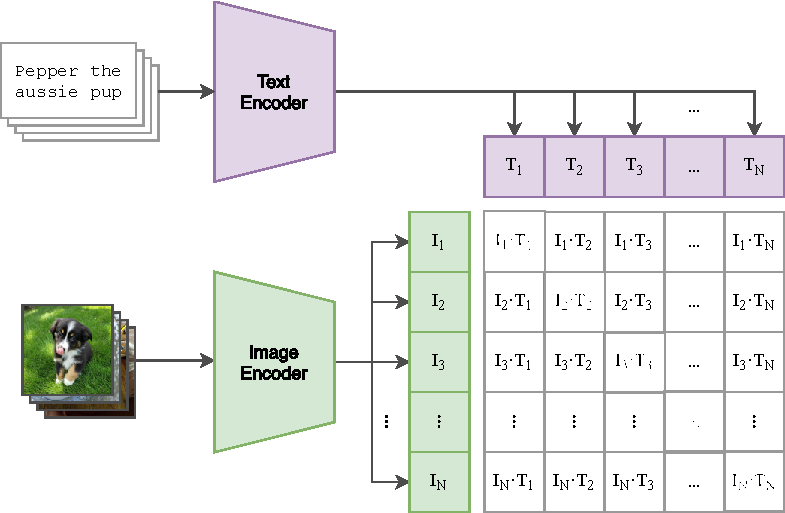
\includegraphics[scale = .7]{imagen-texto}
				\caption{Asignación de textos a imágenes \cite{clip}}
				\label{fig:textos_imagenes}
			\end{figure}
			
			Existen diversas arquitecturas de transformers multimodales capaces de trabajar con imágenes y texto, aunque la forma lograr codificar en embeddings conceptos similares representados de manera diferente, no deja de ser trabajo de los algoritmos de atención múltiple y múltiple-cruzada (\Cref{algo:attention_multiple,algo:attention_multiple-cruzada}). Dependiendo de la arquitectura, existen diferentes variantes del algoritmo de atención múltiple-cruzada (\Cref{fig:variantes_crossed}), aunque el objetivo en todos los casos es el mismo, mezclar y fusionar los embeddings de la imagen y el texto para poder establecer relaciones entre datos aparentemente distintos \cite{multimodal_transformers}. 
			
			\begin{figure}[!h]
				\centering
				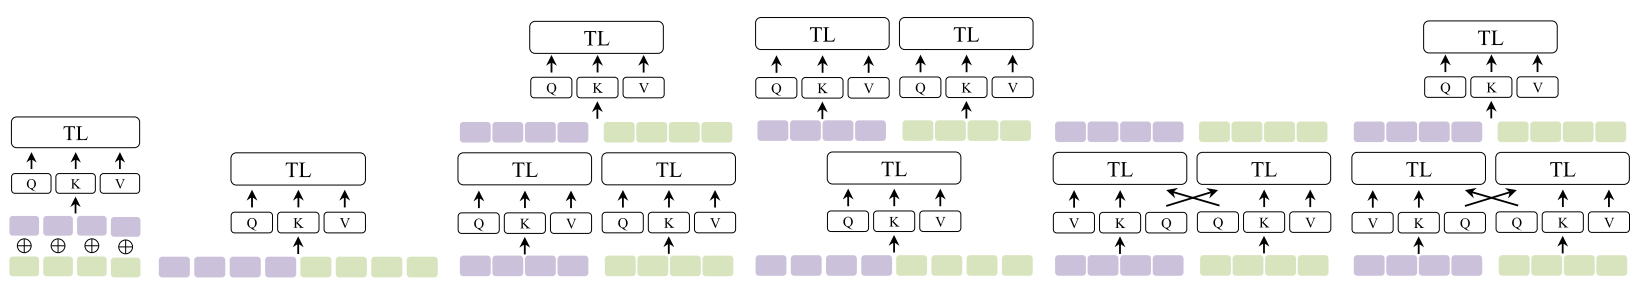
\includegraphics[width = \textwidth]{variantes_crossed}
				\caption{Variantes del algoritmo de atención múltiple-cruzada \cite{multimodal_transformers}}
				\label{fig:variantes_crossed}
			\end{figure}
			
			\subsection{Clasificación no supervisada}
			
				En este punto queda una pregunta por responder. ¿Cómo se realiza la clasificación de textos, imágenes, vídeos, u otras modalidades de información sin conocer el número de clases adecuado y sin tener que modificar la arquitectura del modelo? En general, los transformers con codificador orientados a tareas de clasificación, cuentan con el \gls{cls}, que en el caso de los \gls{vit} originales entregan a una red neuronal clásica, pues no deja de ser un vector $d_m-$dimensional. Al no conocer las clases ni cuántas hay, un posible enfoque es sustituir la red neuronal por un algoritmo de clasificación no supervisada. \\
				
				Uno de los más conocidos es el algoritmo $k-$medias \cite{kmeans} o $k-$means en inglés. Dado un número $k$ de clusters o clases, dicho algoritmo es capaz de clasificar una serie de $n$ elementos $\textbf{x}_i \in \mathbb{R}^d$ en $k$ clases sin conocimiento previo. Para ello, fija de manera aleatoria $k$ puntos $\boldsymbol{\mu}_i \in \mathbb{R}^d$ llamados centroides, que representan el centro de cada cluster. Durante cada iteración, se valora si algún elemento debe cambiar de cluster en función de su distancia a los centroides, y se recalcula la posición de cada uno de ellos. De manera formal, se realiza una partición del dataset $S$ en $k$ conjuntos de manera que 
				$$
				\bigcup_{i = 1}^k S_i = S, \, \bigcap_{i = 1}^k S_i = \varnothing, \text{ y } S_i \neq \varnothing
				$$
				con el fin de minimizar el \gls{wcss}, es decir, 
				$$
				\argmin_{S_1, \ldots, S_k}\sum_{i = 1}^k\sum_{\textbf{x}\in S_i}\|\textbf{x}-\boldsymbol{\mu}_i\|^2. 
				$$ 
				
				Este proceso se describe en el \Cref{algo:kmeans}. El criterio de parada no es único, también se puede elegir un umbral $\varepsilon$. Dicho umbral podría ser un número máximo de iteraciones, una distancia de cambio de los centroides, etc. 
				
				\begin{algorithm}[!h]
					\SetProgSty{texttt}\DontPrintSemicolon
					
					\caption{$k-$means}
					\label{algo:kmeans}
					
					\Datos{$S, k$}
					\Resultado{$S_1, S_2, \hdots, S_k$}
					\textbf{partir} $S$ aleatoriamente\\
					\Repetir{$\forall i\in [1, k]\, S_i(t) \neq S_i(t+1)$}{
						\Para{$i \gets 1$ \KwTo $k$}{
							$S_i(t) \gets \{\textbf{x}:\|\textbf{x}-\boldsymbol{\mu}_i(t)\|^2\leq\|\textbf{x}-\boldsymbol{\mu}_j(t)\|^2\,\land\,\textbf{x}\not\in S_l(t),\,\forall (j, l) \in [1, k] \times [1, i]\}$\\ 
							$\boldsymbol{\mu}_i(t+1) \gets \dfrac{1}{|S_i(t)|}\displaystyle\sum_{\textbf{x}\in S_i}\textbf{x}$
						}
					}
				\end{algorithm}
				
				Otro de los algoritmos de clasificación no supervisada más popular es el de clusterización jerárquica aglomerativa. La traza de este algoritmo crea un árbol comúnmente llamado dendrograma (\Cref{fig:dendro}), que representa una clasificación de los elementos del dataset \cite{ahc}. 
				
				\begin{figure}[!h]
					\Tree[.$S_3$ $x_1$ [.$S_1$ $x_3$ $x_2$ ] [.$S_2$ $x_4$ $x_5$ ] ]
					\caption{Dendrograma}
					\label{fig:dendro}
				\end{figure}
				
				Para lograr la partición del dataset de $n$ elementos en $k$ clusters (con $k \leq n$), inicialmente cada elemento se encuentra en un cluster distinto y durante las iteraciones del algoritmo se van uniendo los clusters más próximos, y determinando la distancia entre estos mediante una función. Existen multitud de ellas, dando lugar a variantes del algoritmo como single, complete, average, Ward, etc. \cite{ahc_variantes}\\
				
				\begin{algorithm}
					\SetProgSty{texttt}\DontPrintSemicolon
					
					\caption{Clustering jerárquico aglomerativo}
					\label{algo:ahc}
					
					\Datos{$S, k$}
					\Resultado{$S_1, S_2, \hdots, S_k$}
					$\forall i \, S_i \gets \{\textbf{x}_i\}$\\
					\Para{$j \gets n$ \KwTo $k$}{
						$D \in \mathbb{R}^{j \times j}$\\ 
						$\forall(p,q)\,D_{pq} \gets \text{dist}(S_p, S_q)$\\
						$l, m = \displaystyle\argmin_{a, b}D_{ab}$\\
						$S_l \gets S_l \cup S_m$\\
						\textbf{eliminar} $S_m$
					}
				\end{algorithm}
				
				Una característica que tienen en común estos dos algoritmos es que, si bien no necesitan de conocimiento previo para realizar la clasificación, sí necesitan conocer el número de clases. En el caso que no se tiene conocimiento suficiente sobre el dataset para poder determinar el valor óptimo de clases, se puede utilizar el conocido como método del codo o rodilla. Este método propone utilizar $k-$means para determinar el $k$ óptimo, tomando aquel que genere un punto que sería el codo en una gráfica que represente cada \gls{wcss} para cada $k$, que tendría forma de brazo \cite{elbow}, tal y como describe el \Cref{algo:codo}. \\
				
				\begin{figure}[!h]
					\centering
					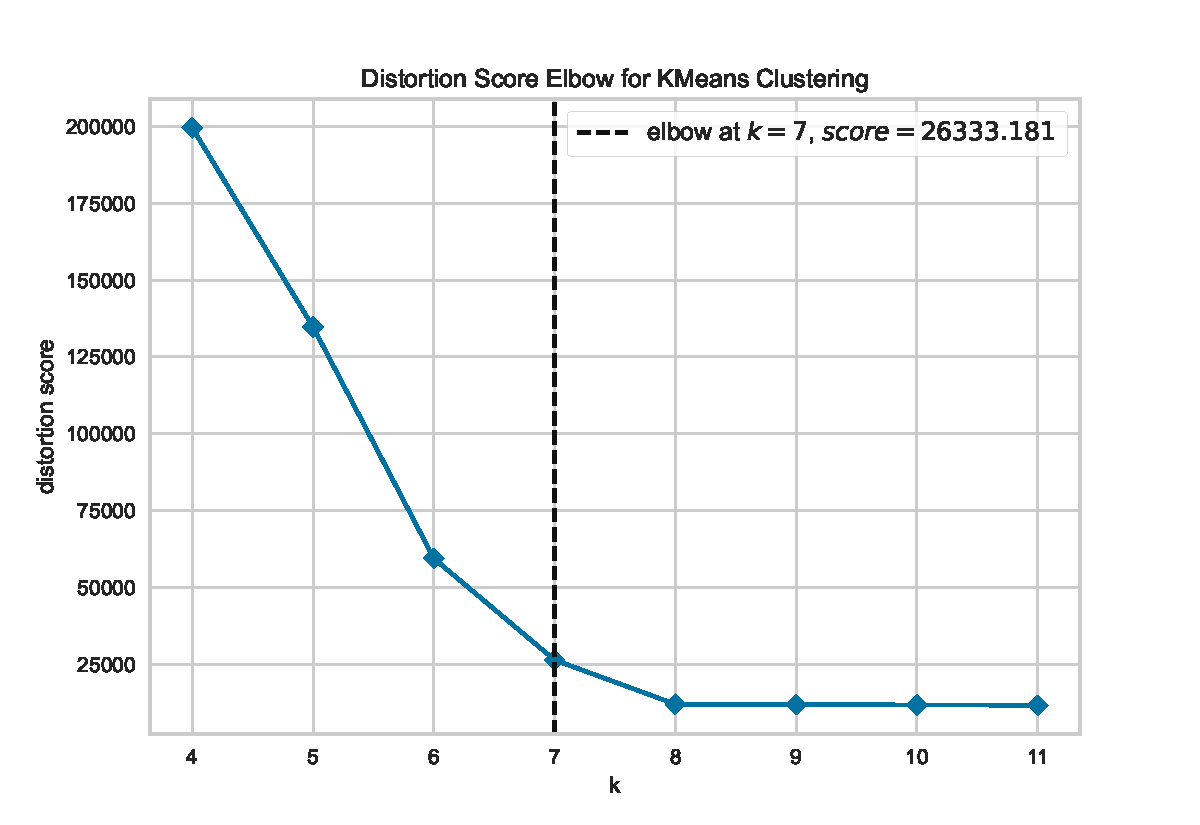
\includegraphics[scale = .35]{elbow_ejemplo}
					\caption{$k$ óptimo mediante el método del codo}
					\label{fig:ejemplo_codo}
				\end{figure}
				
				\begin{algorithm}[!h]
					\SetProgSty{texttt}\DontPrintSemicolon
					
					\caption{Método del codo}
					\label{algo:codo}
					
					\Datos{$S, k, a, b$}
					\Resultado{$k'$}
					$\textbf{s} \in \mathbb{R}^n$\\
					$\textbf{d} \in \mathbb{R}^n$\\
					\Para{$i \gets a$ \KwTo $n$}{
						$\boldsymbol{\mu} \gets k-\text{means}(S, k)$\\
						$s_i \gets \displaystyle\sum_{j = 1}^k\sum_{\textbf{x}\in S_j}\|\textbf{x}-\boldsymbol{\mu}_j\|^2$\\
						$k_i \gets i$
					}
					$k' \gets$ kneedle$(\textbf{k}, \textbf{s})$
				\end{algorithm}
				
				
				La cuestión que queda por resolver es cómo ``calcular el codo''. Este punto se suele definir como el de mayor curvatura, por lo que si dada una serie de valores $\textbf{s}$ de \gls{wcss}, mediante una función $\mathcal{K}(k, y)$ se pudiese calcular la curvatura en ese punto, bastaría con tomar el $k$ que maximice $\mathcal{K}(k, y)$. Para realizar esta tarea se suele utilizar el llamado algoritmo \textit{kneedle}. Dicho nombre proviene del juego de palabras knee (rodilla) y needle (aguja), que en el título de la publicación original \cite{kneedle}, se compara con buscar una aguja en un pajar. Tal y como muestra el \Cref{algo:kneedle}, la idea es normalizar los valores, y tomar como punto de curvatura máxima aquel $x$ que maximiza $f(x) - x$. Se puede fijar un umbral para evitar máximos locales. 
				
				\begin{figure}[!h]
					\centering
					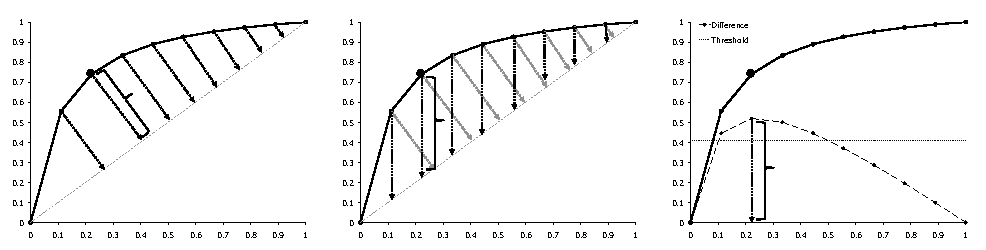
\includegraphics[width = \textwidth]{kneedle}
					\caption{Punto de mayor curvatura mediante Kneedle}
					\label{fig:kneedle}
				\end{figure}
				
				\begin{algorithm}
					\DontPrintSemicolon
					
					\caption{Kneedle}
					\label{algo:kneedle}
					
					\Datos{$\textbf{s}, \textbf{k}$}
					\Resultado{$k'$}
					$\textbf{d} \in \mathbb{R}^n$\\
					\Para{$i \gets \min\{\mathbf{k}\}$ \KwTo $\max\{\mathbf{k}\}$}{
						$s_i' \gets \dfrac{s_i - \min\{\textbf{s}\}}{\max\{\textbf{s}\}-\min\{\textbf{s}\}}$\\
						$k_i' \gets \dfrac{k_i - \min\{\textbf{\textbf{k}}\}}{\max\{\textbf{k}\}-\min\{\textbf{k}\}}$\\
						$d_i \gets s_i' - k_i$
					}
					$k' \gets \displaystyle\argmax \textbf{d}$
				\end{algorithm}